%%%%%%%%%%%%%%%%%%%%%%%%%%%%%%%%%%%%%%%%%%%%%%%%%%%%%%%%%%%%%%%%%%%%%%%%%%%%%%
%  PairCLIP-SWA: Semantic Pair Mining and Stochastic Weight Averaging for
%  Generalized Deepfake Image Detection with OpenCLIP Vision Transformers
%%%%%%%%%%%%%%%%%%%%%%%%%%%%%%%%%%%%%%%%%%%%%%%%%%%%%%%%%%%%%%%%%%%%%%%%%%%%%%
\documentclass[10pt,journal]{IEEEtran}

\usepackage{amsmath,amssymb,amsfonts,mathtools}
\usepackage{graphicx}
\usepackage{booktabs}
\usepackage{multirow}
\usepackage{array}
\usepackage{threeparttable}
\usepackage{makecell}
\usepackage{xcolor}
\usepackage{algorithm}
\usepackage{algpseudocode}
\usepackage{tikz}
\usetikzlibrary{arrows.meta,positioning,calc,fit,backgrounds,shapes.geometric}
\usepackage{balance}
\usepackage{url}
\usepackage[hidelinks,breaklinks=true]{hyperref}
\usepackage{cite}

% ---- convenience macros -------------------------------------------------
\newcommand{\vect}[1]{\boldsymbol{#1}}
\newcommand{\mat}[1]{\mathbf{#1}}
\newcommand{\real}{\mathbb{R}}
\newcommand{\Ex}{\mathbb{E}}
\newcommand{\bs}{\vspace{2pt}}
\DeclareMathOperator*{\argmax}{arg\,max}
\DeclareMathOperator*{\argmin}{arg\,min}
\newcommand{\best}[1]{\textbf{#1}}
\newcommand{\pct}{\%}

% ---- table helpers ------------------------------------------------------
\newcolumntype{L}[1]{>{\raggedright\arraybackslash}p{#1}}
\newcolumntype{C}[1]{>{\centering\arraybackslash}p{#1}}
\newcolumntype{R}[1]{>{\raggedleft\arraybackslash}p{#1}}

\hyphenation{deep-fake deep-fakes Open-CLIP}

\begin{document}

\title{PairCLIP-SWA: Semantic Pair Mining and\\
Stochastic Weight Averaging for Generalized\\
Deepfake Image Detection with OpenCLIP}

\author{Md.~Nakib,
        Sudipto~Sarkar,
        A.~J.~A.~Jubayer~Talukder,
        and~Arif~Mahmud\\[4pt]
\normalsize Department of Electrical and Electronic Engineering,\\
\normalsize BUET, Dhaka 1205, Bangladesh% <-this % stops a space
\thanks{Manuscript prepared August 2026.}}

\markboth{Manuscript submitted for publication}%
{Nakib \MakeLowercase{\textit{et al.}}: PairCLIP-SWA for Generalized Deepfake Image Detection}

\IEEEtitleabstractindextext{%
\begin{abstract}
Deepfake detectors routinely exceed 99\% accuracy on the generator family they
were trained on, yet collapse when confronted with unseen manipulation
pipelines. The IEEE Signal Processing Cup 2025 (DF-Wild-Cup) corpus was
constructed to expose exactly this failure, and the strongest published result
on it is obtained by a three-backbone convolution--attention ensemble that
fuses spatial and wavelet-domain evidence. We ask whether comparable or better
generalization can be reached with a \emph{single} backbone by changing what
the model is trained on rather than how many models are averaged. We propose
PairCLIP-SWA, a three-stage framework. First, a frozen CLIP ViT-L/14 encoder
mines a one-to-one semantic correspondence between the real and fake pools by
approximately solving a maximum-weight bipartite matching in cosine-similarity
space; the resulting corpus is balanced not only in class \emph{counts} but in
class-conditional \emph{content}, which removes identity, pose and scene
shortcuts from the learning signal. Second, an OpenCLIP ViT-L/14 visual tower
is adapted through a progressively widening block-unfreezing schedule with a
linear head, a class-balanced paired sampler, and mixed-precision training.
Third, stochastic weight averaging collapses the fine-tuning trajectory into a
single flat-minimum solution. Without a single gradient step on DF-Wild-Cup
training data, PairCLIP-SWA attains \best{97.04\%} on the official 3{,}072-image
validation set, against 94.46\% for the published ensemble --- a 46.5\%
relative reduction in error. On a 39{,}428-image OpenForensics-derived
benchmark it converges within eleven epochs to 98.64\% validation accuracy at
98.46\% training accuracy, a gap of 0.18 points indicating regularization
rather than memorization. On the disjoint 10{,}905-image held-out test
partition the validation-selected checkpoint nevertheless falls to 88.85\%,
with 94.0\% of its errors being genuine photographs rejected as forgeries,
while the terminal weight average recovers \best{94.76\%} and rebalances the
error budget --- a 53.0\% reduction in test error. We therefore report a
methodological result alongside the empirical one: validation accuracy selected
the checkpoint that makes twice as many deployment errors, and forensic
detectors should be chosen on per-class criteria measured off the
early-stopping split.
\end{abstract}

\begin{IEEEkeywords}
Deepfake detection, vision--language models, CLIP, OpenCLIP, vision
transformer, transfer learning, stochastic weight averaging, bipartite
matching, class balancing, t-SNE, cluster separability, media forensics.
\end{IEEEkeywords}}

\maketitle
\IEEEdisplaynontitleabstractindextext
\IEEEpeerreviewmaketitle

% =========================================================================
\section{Introduction}
% =========================================================================
\IEEEPARstart{T}{he} industrialization of generative modelling has made
photorealistic face synthesis a commodity. Generative adversarial
networks~\cite{goodfellow2014gan,karras2020stylegan2} and, more recently,
latent diffusion models~\cite{rombach2022ldm} place convincing identity
manipulation within reach of any user with a consumer GPU. The forensic
consequences are well documented: non-consensual imagery, financial fraud,
and coordinated political disinformation~\cite{verdoliva2020media,
tolosana2020survey}. Detection has therefore become a safety-critical signal
processing problem.

The literature reports a persistent and awkward pattern. Detectors trained and
tested within a single manipulation family are close to saturated, while the
same detectors degrade towards chance when the generator changes, when the
compression pipeline changes, or when the acquisition conditions
change~\cite{wang2020cnngenerated,corvi2023diffusion}. The community response
has been to enlarge the hypothesis class: frequency-domain
branches~\cite{frank2020frequency,durall2020upconvolution,qian2020f3net},
attention pooling~\cite{zhao2021multiattentional}, and heterogeneous ensembles
that combine convolutional, transformer and wavelet
experts~\cite{bhattacharjee2026caenet,gowda2022ensemble}. The IEEE Signal
Processing Cup 2025 (DF-Wild-Cup) corpus was assembled specifically to
stress-test this regime: it merges eight standard deepfake benchmarks under
the DeepfakeBench preprocessing protocol~\cite{yan2023deepfakebench}, strips
provenance metadata, and presents a $5{:}1$ fake-to-real imbalance. The
strongest published result on this corpus, CAE-Net~\cite{bhattacharjee2026caenet},
reaches $94.46\%$ accuracy by fusing EfficientNet-B0~\cite{tan2019efficientnet},
DeiT~\cite{touvron2021deit} and a wavelet-fed ConvNeXt~\cite{liu2022convnext}
through a tuned late-fusion rule, at a cost of $117.4$\,M parameters, five
sequential training stages, and three forward passes per query image.

\subsection{Research Gaps}
We identify three gaps that motivate this work.

\textbf{G1: Narrow pre-training priors.} Nearly all detectors reported on
DF-Wild-Cup, CAE-Net included, initialize from ImageNet-supervised
weights~\cite{deng2009imagenet}. ImageNet supervision optimizes a
$1000$-way object-category posterior; the resulting features are excellent
object detectors but carry a comparatively narrow prior over the appearance
statistics of \emph{people, scenes and capture conditions} in the wild.
Contrastive image--text pre-training on web-scale
corpora~\cite{radford2021clip,cherti2023openclip,schuhmann2022laion5b} yields
representations whose transfer profile is markedly broader, and several recent
works confirm that CLIP features alone separate synthetic from natural imagery
across generator families that were never
observed~\cite{ojha2023universal,cozzolino2024raising,khan2024clipping}.
However, naive linear probing of frozen CLIP under-fits the fine-grained,
high-frequency evidence that forensics requires, while unconstrained
end-to-end fine-tuning is known to distort exactly the pre-trained geometry
that provides out-of-distribution robustness~\cite{kumar2022finetuning}. The
right amount of adaptation is an open design question.

\textbf{G2: Balancing counts is not balancing content.} Class imbalance in
deepfake corpora is universally treated as a \emph{counting} problem, addressed
by oversampling, synthetic minority generation~\cite{chawla2002smote}, loss
reweighting, or --- as in CAE-Net --- partitioning the majority class into
disjoint subsets. All of these equalize $|\mathcal{R}|$ and $|\mathcal{F}|$
while leaving the class-conditional \emph{content} distributions
$p(\text{content}\mid\text{real})$ and $p(\text{content}\mid\text{fake})$
free to differ. When they do differ --- different identities, poses,
backgrounds, or illumination in the two pools --- a discriminative model can
lower its training loss by keying on content rather than on manipulation
traces. Such a shortcut is invisible in-distribution and catastrophic
out-of-distribution.

\textbf{G3: Single-checkpoint selection is fragile.} Fine-tuned vision
transformers traverse wide, flat regions of the loss surface, so the
validation accuracy of individual checkpoints along a trajectory fluctuates by
more than a percentage point. Reporting the single best checkpoint both
overstates the expected accuracy and discards the information contained in the
rest of the trajectory. Weight-space averaging is an established remedy in
generic
classification~\cite{izmailov2018swa,wortsman2022soups} but has not, to our
knowledge, been evaluated on a cross-corpus deepfake benchmark.

\subsection{Contributions}
This paper makes the following contributions.

\begin{enumerate}
\item \textbf{CLIP-guided semantic pair mining.} We formulate the construction
of a content-balanced training corpus as a maximum-weight bipartite matching
between real and fake images in the cosine-similarity space of a frozen CLIP
ViT-L/14 encoder, and solve it with a memory-bounded greedy approximation that
runs in $O(n_r n_f)$ time and $O(B n_f)$ memory (Section~\ref{sec:pairing}).
The result is a corpus in which the class label is, by construction,
approximately independent of semantic content.

\item \textbf{A paired, class-exact sampler.} We pair the mined corpus with a
batch sampler that interleaves the two class index streams, guaranteeing an
exact $1{:}1$ class ratio in \emph{every} mini-batch rather than in
expectation (Section~\ref{sec:sampler}).

\item \textbf{Progressive block unfreezing of an OpenCLIP tower.} We adapt an
OpenCLIP ViT-L/14 visual encoder with a monotonically widening unfreezing
schedule, $k(e)=\min(2+\lfloor e/2 \rfloor, K_{\max})$ transformer blocks at
epoch $e$, capped at $K_{\max}=14$ of $24$ blocks
(Section~\ref{sec:unfreeze}). This interpolates between linear probing and
full fine-tuning and keeps $41.98\%$ of the backbone --- the patch embedding,
the positional code and the first ten blocks --- permanently frozen.

\item \textbf{Stochastic weight averaging for forensic transfer.} We average
the fine-tuning trajectory in weight space with a constant reduced learning
rate (Section~\ref{sec:swa}). On the hardest of our three benchmarks this
converts a $95.67\%$ best-checkpoint result into $97.04\%$, a gain of $1.37$
percentage points at zero inference cost.

\item \textbf{Quantitative embedding-geometry analysis.} Beyond accuracy, we
characterize the learned representation with an inter-centroid separation
score and a k-NN probe on the t-SNE embedding of the DF-Wild-Cup validation
set (Sections~\ref{sec:cluster-method} and~\ref{sec:cluster-results}), and
report the counter-intuitive finding that weight averaging \emph{reduces}
raw cluster separation while \emph{improving} both probe and classifier
accuracy.

\item \textbf{Cross-corpus evaluation against a published benchmark.}
PairCLIP-SWA reaches $97.04\%$ on the official DF-Wild-Cup validation split
\emph{without taking a single gradient step on DF-Wild-Cup training images},
versus $94.46\%$ for an ensemble trained in-domain on that corpus
(Section~\ref{sec:spcup}).

\item \textbf{Evidence that validation accuracy misranks forensic
detectors.} On a $10{,}905$-image held-out partition used for neither
gradients nor selection, the validation-selected checkpoint reaches $88.85\%$
while the checkpoint that validation accuracy ranks \emph{last} reaches
$94.76\%$ (Section~\ref{sec:test}). The failure is entirely one-sided ---
specificity falls to $78.88\%$ while fake-class recall is retained at
$98.67\%$ --- and is invisible to scalar accuracy on a balanced split. We
recommend per-class selection criteria measured off the early-stopping
partition.
\end{enumerate}

\subsection{Organization}
Section~\ref{sec:related} surveys related work. Section~\ref{sec:method}
develops the proposed methodology, including the formal treatment of pair
mining, the backbone, the optimization routine and the clustering framework.
Section~\ref{sec:exp} describes the experimental protocol and reports results
on three datasets together with the head-to-head comparison against CAE-Net.
Section~\ref{sec:discussion} provides ablation, complexity analysis, critical
discussion and limitations. Section~\ref{sec:conclusion} concludes.

% =========================================================================
\section{Related Work}\label{sec:related}
% =========================================================================

\subsection{Spatial-Domain Deepfake Detection}
Early detectors treated forgery detection as ordinary binary classification
over CNN backbones such as VGG~\cite{simonyan2015vgg},
ResNet~\cite{he2016resnet}, Xception~\cite{chollet2017xception} and
EfficientNet~\cite{tan2019efficientnet}, and this line still provides the
strongest single-model baselines on face-swap corpora such as
FaceForensics++~\cite{rossler2019faceforensics} and
Celeb-DF~\cite{li2020celebdf}. Refinements add attention: squeeze-and-excitation
recalibration~\cite{hu2018senet}, convolutional block attention~\cite{woo2018cbam},
and multi-attentional pooling over local artifact
maps~\cite{zhao2021multiattentional}. Wang \emph{et al.}~\cite{wang2020cnngenerated}
showed that a single ProGAN-trained classifier transfers surprisingly well
across CNN generators given aggressive augmentation, but Corvi \emph{et
al.}~\cite{corvi2023diffusion} demonstrated that the same recipe fails on
diffusion imagery, re-opening the generalization question.

\subsection{Frequency-Domain and Hybrid Detection}
Up-sampling operators in generative decoders leave periodic spectral
signatures~\cite{durall2020upconvolution}, which motivated detectors operating
on the DCT~\cite{frank2020frequency,ricker2024dct}, on learned frequency
bands~\cite{qian2020f3net}, and on wavelet
packets~\cite{wolter2022waveletpacket}. These cues are sharp but fragile:
re-compression, resizing and denoising attenuate them. Consequently the strongest
recent systems are hybrids. CAE-Net~\cite{bhattacharjee2026caenet}, the reference
point for this paper, combines EfficientNet-B0 for local artifacts, DeiT-B for
global context, and a ConvNeXt fed with single-level Haar 2D-DWT coefficients,
fusing the three at probability level. It also introduces a disjoint-subset
multistage schedule that splits the $219{,}470$ fake images of DF-Wild-Cup into
five non-overlapping subsets, each trained jointly with the full $42{,}690$-image
real set and warm-started from the previous stage. Our work shares CAE-Net's
diagnosis --- balance and diversity are what matter --- but differs in the
remedy: we balance content through matching rather than counts through
partitioning, and we replace the ensemble with one vision--language backbone.

\subsection{CLIP and Vision--Language Models for Forensics}
CLIP~\cite{radford2021clip} and its open reproduction
OpenCLIP~\cite{ilharco2021openclip,cherti2023openclip} learn a joint
image--text embedding from hundreds of millions of web pairs. Ojha \emph{et
al.}~\cite{ojha2023universal} observed that a nearest-neighbour or linear
classifier on \emph{frozen} CLIP features generalizes across generator
families far better than a fine-tuned CNN, arguing that the pre-trained
manifold is not specialized to any particular synthesis artifact. Cozzolino
\emph{et al.}~\cite{cozzolino2024raising} strengthened this result with careful
augmentation and calibration, and Khan and
Dang-Nguyen~\cite{khan2024clipping} systematically compared adaptation
strategies --- linear probing, prompt tuning, adapters and full fine-tuning ---
for universal deepfake detection. Our design sits between the extremes these
works bracket: we neither freeze the tower nor fine-tune it entirely, but
unfreeze a growing suffix of transformer blocks, which is the configuration
that the feature-distortion analysis of Kumar \emph{et
al.}~\cite{kumar2022finetuning} predicts should retain out-of-distribution
robustness while still fitting forensic evidence. Gradual unfreezing itself
originates in transfer learning for NLP~\cite{howard2018ulmfit}.

\subsection{Data Construction and Pairing}
Pairing is a recurring motif in forensics. Self-blended
images~\cite{shiohara2022sbi} synthesize a pseudo-fake from a single source
frame, so that the real and fake members of a pair share identity exactly and
differ only in the blending boundary. This is precisely the content-balancing
argument of gap G2, but it requires a synthesis operator and therefore biases
the fake distribution towards the artifacts of that operator. Our pair mining
is complementary: it \emph{discovers} correspondences inside an existing,
generator-agnostic corpus rather than manufacturing them, at the cost of only
approximate content alignment. Formally the discovery step is an assignment
problem~\cite{kuhn1955hungarian,burkard2012assignment}, for which we use a
greedy approximation for tractability at corpus scale.

\subsection{Weight Averaging and Flat Minima}
Stochastic weight averaging~\cite{izmailov2018swa} maintains a running mean of
the iterates visited under a high constant learning rate and converges to
wider optima with better generalization; model soups~\cite{wortsman2022soups}
extend the idea to independently fine-tuned runs. Both are essentially free at
inference time, which makes them attractive precisely where ensembles are not.
We apply SWA to a partially unfrozen vision--language tower and evaluate it in
a cross-corpus forensic setting, a combination we have not found in the
deepfake literature.

% =========================================================================
\section{Proposed Methodology}\label{sec:method}
% =========================================================================

\begin{figure*}[!t]
\centering
\resizebox{0.99\textwidth}{!}{%
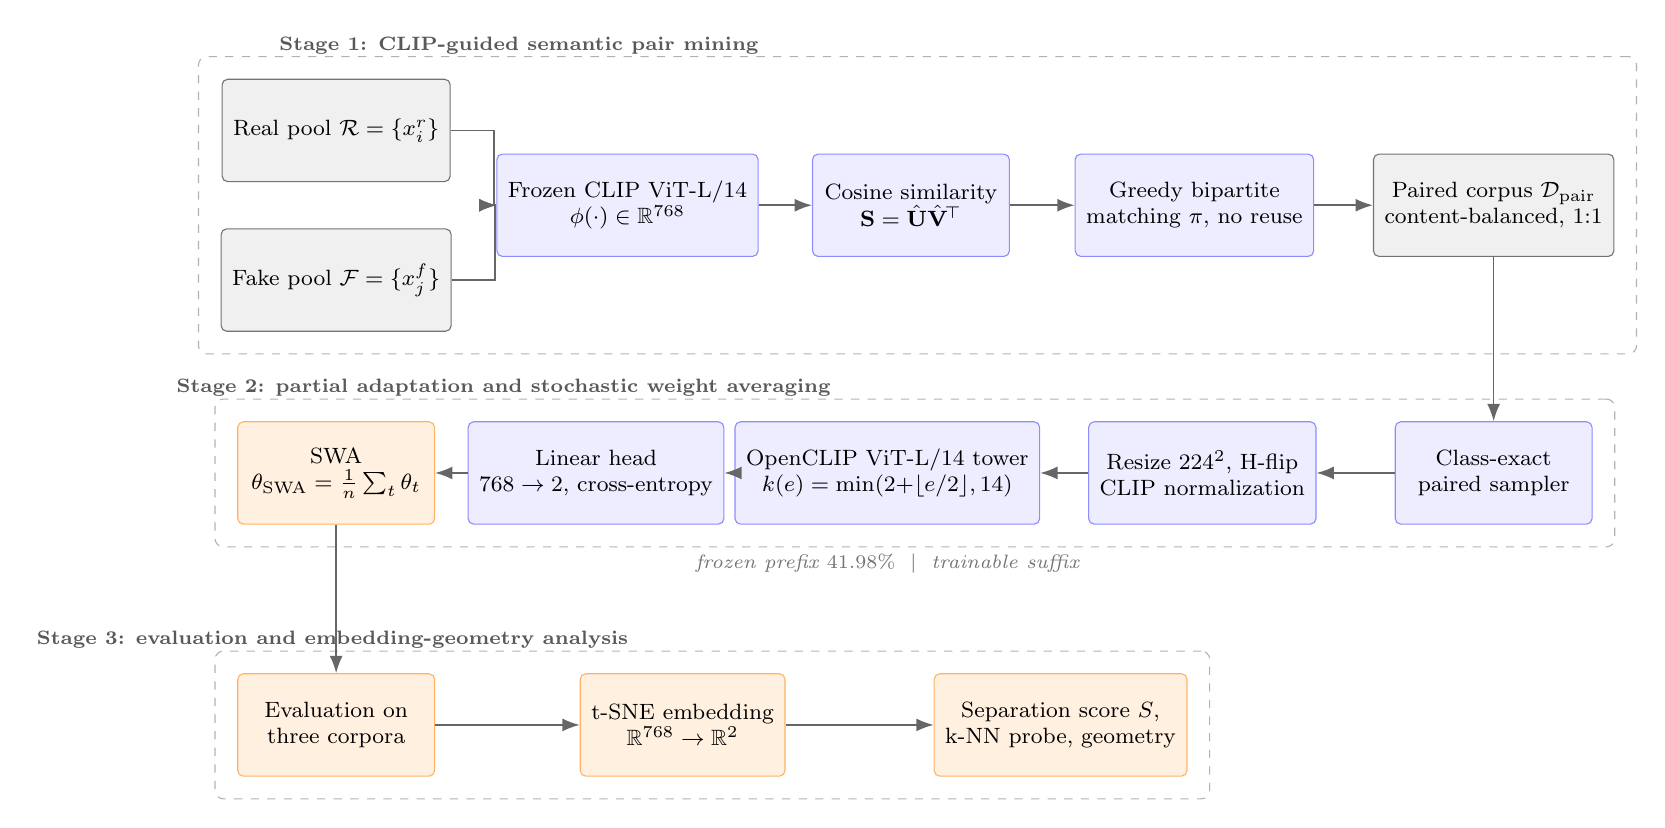
\begin{tikzpicture}[
  font=\footnotesize,
  nbox/.style ={draw=black!55,rounded corners=2pt,align=center,inner sep=4pt,
                minimum height=13mm,minimum width=25mm,fill=white},
  ndata/.style={nbox,fill=black!6},
  nproc/.style={nbox,fill=blue!7,draw=blue!45},
  nres/.style ={nbox,fill=orange!12,draw=orange!60},
  narr/.style ={-{Latex[length=2.2mm]},draw=black!60,line width=0.6pt},
  nlbl/.style ={font=\scriptsize\itshape,text=black!55}
]
% ---------------- Stage 1 (left to right) ----------------
\node[ndata] (real)  at (0,0.95) {Real pool $\mathcal{R}=\{x^r_i\}$};
\node[ndata] (fake)  at (0,-0.95) {Fake pool $\mathcal{F}=\{x^f_j\}$};
\node[nproc] (clip)  at (3.7,0)  {Frozen CLIP ViT-L/14\\$\phi(\cdot)\in\real^{768}$};
\node[nproc] (sim)   at (7.3,0)  {Cosine similarity\\$\mat{S}=\hat{\mat{U}}\hat{\mat{V}}^{\!\top}$};
\node[nproc] (match) at (10.9,0) {Greedy bipartite\\matching $\pi$, no reuse};
\node[ndata] (corpus)at (14.7,0) {Paired corpus $\mathcal{D}_{\mathrm{pair}}$\\content-balanced, $1{:}1$};

\draw[narr] (real.east)  -- ++(0.55,0) |- (clip.west);
\draw[narr] (fake.east)  -- ++(0.55,0) |- (clip.west);
\draw[narr] (clip)  -- (sim);
\draw[narr] (sim)   -- (match);
\draw[narr] (match) -- (corpus);

% ---------------- Stage 2 (right to left) ----------------
\node[nproc] (sampler) at (14.7,-3.4) {Class-exact\\paired sampler};
\node[nproc] (aug)     at (11.0,-3.4) {Resize $224^2$, H-flip\\CLIP normalization};
\node[nproc] (tower)   at (7.0,-3.4)  {OpenCLIP ViT-L/14 tower\\$k(e)=\min(2{+}\lfloor e/2\rfloor,14)$};
\node[nproc] (head)    at (3.3,-3.4)  {Linear head\\$768\to2$, cross-entropy};
\node[nres]  (swa)     at (0,-3.4)    {SWA\\$\theta_{\mathrm{SWA}}=\frac{1}{n}\sum_t\theta_t$};

\draw[narr] (corpus)  -- (sampler);
\draw[narr] (sampler) -- (aug);
\draw[narr] (aug)     -- (tower);
\draw[narr] (tower)   -- (head);
\draw[narr] (head)    -- (swa);
\node[nlbl] at (7.0,-4.55) {frozen prefix $41.98\%$ $\;\vert\;$ trainable suffix};

% ---------------- Stage 3 (left to right) ----------------
\node[nres] (eval)    at (0,-6.6)   {Evaluation on\\three corpora};
\node[nres] (tsne)    at (4.4,-6.6) {t-SNE embedding\\$\real^{768}\to\real^{2}$};
\node[nres] (metrics) at (9.2,-6.6) {Separation score $S$,\\k-NN probe, geometry};

\draw[narr] (swa)  -- (eval);
\draw[narr] (eval) -- (tsne);
\draw[narr] (tsne) -- (metrics);

\begin{scope}[on background layer]
\node[fit=(real)(fake)(corpus),draw=black!30,dashed,rounded corners=3pt,
      inner sep=8pt,
      label={[font=\scriptsize\bfseries,text=black!65,yshift=-1mm]above left:%
      Stage 1: CLIP-guided semantic pair mining}] {};
\node[fit=(swa)(sampler),draw=black!30,dashed,rounded corners=3pt,
      inner sep=8pt,
      label={[font=\scriptsize\bfseries,text=black!65,yshift=-1mm]above left:%
      Stage 2: partial adaptation and stochastic weight averaging}] {};
\node[fit=(eval)(metrics),draw=black!30,dashed,rounded corners=3pt,
      inner sep=8pt,
      label={[font=\scriptsize\bfseries,text=black!65,yshift=-1mm]above left:%
      Stage 3: evaluation and embedding-geometry analysis}] {};
\end{scope}
\end{tikzpicture}}
\caption{Overview of the PairCLIP-SWA framework. Stage~1 uses a frozen CLIP
ViT-L/14 encoder to mine a one-to-one semantic correspondence between the real
and fake pools, producing a corpus that is balanced in class counts \emph{and}
in class-conditional content. Stage~2 adapts an OpenCLIP ViT-L/14 visual tower
with a progressively widening unfreezing schedule and a linear head, trained
with class-exact paired batches, and collapses the trajectory with stochastic
weight averaging. Stage~3 evaluates the resulting detector on three corpora and
characterizes its embedding geometry.}
\label{fig:pipeline}
\end{figure*}

\subsection{Problem Statement and Notation}
Let $\mathcal{X}$ denote the space of RGB face images and $y\in\{0,1\}$ a
binary authenticity label. Throughout this paper we adopt the convention
$y=1$ for \emph{real} and $y=0$ for \emph{fake}, matching our implementation;
where we quote metrics from~\cite{bhattacharjee2026caenet} we treat the
\emph{fake} class as positive, as those authors do, and state the convention
explicitly. We are given a training corpus drawn from a source distribution
$p_{\mathcal{S}}$ and must produce a classifier $f_\theta:\mathcal{X}\to\{0,1\}$
whose risk is small under a \emph{different} target distribution
$p_{\mathcal{T}}$ that contains manipulation families absent from
$p_{\mathcal{S}}$. Write $\mathcal{R}=\{x^r_i\}_{i=1}^{n_r}$ and
$\mathcal{F}=\{x^f_j\}_{j=1}^{n_f}$ for the real and fake pools of the source
corpus. Figure~\ref{fig:pipeline} summarizes the full framework.

\subsection{Stage 1: CLIP-Guided Semantic Pair Mining}\label{sec:pairing}

\subsubsection{Motivation}
Decompose each image into a latent content factor $c$ (identity, pose,
expression, illumination, background, capture pipeline) and a manipulation
factor $m$. A detector minimizing empirical risk on a corpus in which
$p(c\mid y{=}1)\neq p(c\mid y{=}0)$ can achieve low training loss using $c$
alone. Because $c$ is not causally linked to authenticity, any such solution
fails as soon as the target corpus re-couples content and label differently.
Our objective is therefore to construct a subset
$\mathcal{D}_{\mathrm{pair}}\subseteq\mathcal{R}\times\mathcal{F}$ on which
the two class-conditional content distributions are as close as possible.

\subsubsection{Embedding}
We embed every image with a frozen CLIP ViT-L/14 image
encoder~\cite{radford2021clip}, $\phi:\mathcal{X}\to\real^{d}$ with $d=768$.
CLIP's contrastive objective aligns images with natural-language captions, so
$\phi$ is by construction a \emph{semantic} descriptor: cosine proximity in
its output space corresponds to similarity of describable content, and it is
largely insensitive to the low-amplitude, high-frequency residues that
distinguish a manipulated face from its source. This is exactly the property
we require of the matching criterion --- we want to pair images by
\emph{content}, not by \emph{artifact}. Images are resized to $224\times224$
and passed through the standard CLIP preprocessing before embedding. Denote
$\vect{u}_i=\phi(x^r_i)$ and $\vect{v}_j=\phi(x^f_j)$, and let
$\hat{\vect{u}}_i=\vect{u}_i/\lVert\vect{u}_i\rVert_2$,
$\hat{\vect{v}}_j=\vect{v}_j/\lVert\vect{v}_j\rVert_2$.

\subsubsection{Matching Objective}
Stacking the normalized embeddings into
$\hat{\mat{U}}\in\real^{n_r\times d}$ and
$\hat{\mat{V}}\in\real^{n_f\times d}$ gives the similarity matrix
\begin{equation}
\mat{S}=\hat{\mat{U}}\hat{\mat{V}}^{\!\top}\in[-1,1]^{n_r\times n_f},
\qquad
S_{ij}=\frac{\langle\vect{u}_i,\vect{v}_j\rangle}
             {\lVert\vect{u}_i\rVert_2\,\lVert\vect{v}_j\rVert_2}.
\label{eq:sim}
\end{equation}
The ideal pairing is the injective assignment $\pi:\{1,\dots,n_r\}\to
\{1,\dots,n_f\}$ that maximizes total semantic agreement,
\begin{equation}
\pi^\star=\argmax_{\pi\ \text{injective}}\ \sum_{i=1}^{n_r}S_{i,\pi(i)} .
\label{eq:assignment}
\end{equation}
Equation~\eqref{eq:assignment} is a linear assignment
problem~\cite{kuhn1955hungarian,burkard2012assignment}. Its exact solution by
the Hungarian algorithm costs $O(n^3)$ with $n=\max(n_r,n_f)$, which is
prohibitive at corpus scale and, more importantly, unnecessary: we do not need
the optimal matching, only one whose induced content distributions are close.

\subsubsection{Memory-Bounded Greedy Approximation}
We therefore solve~\eqref{eq:assignment} greedily and sequentially. Processing
real images in order, and maintaining the set $\mathcal{U}_{i-1}$ of fake
indices already consumed,
\begin{align}
\pi(i)&=\argmax_{j\notin\mathcal{U}_{i-1}} S_{ij},
\label{eq:greedy}\\
\mathcal{U}_i&=\mathcal{U}_{i-1}\cup\{\pi(i)\},\qquad \mathcal{U}_0=\varnothing .
\end{align}
The without-replacement constraint in~\eqref{eq:greedy} is essential: it
prevents a single visually generic fake image from absorbing thousands of real
partners, which would defeat the purpose of the construction. Greedy matching
of this form is a $\tfrac{1}{2}$-approximation for maximum-weight matching, and
in practice recovers a large fraction of the optimum because $\mat{S}$ is
strongly diagonally dominant after CLIP normalization.

Materializing $\mat{S}$ requires $O(n_r n_f)$ memory, which is infeasible for
corpora of realistic size. We stream the computation in row blocks of size
$B$: for block $b$ we form only $\mat{S}^{(b)}=\hat{\mat{U}}^{(b)}
\hat{\mat{V}}^{\!\top}\in\real^{B\times n_f}$, apply~\eqref{eq:greedy} to its
rows, and release it. Peak memory is thus $O(Bn_f)$ rather than
$O(n_r n_f)$, while total arithmetic is unchanged at $O(n_r n_f d)$ for the
similarities and $O(n_r n_f)$ for the selections. We use $B=1000$.
Algorithm~\ref{alg:pairing} states the procedure.

\begin{algorithm}[!t]
\caption{CLIP-Guided Semantic Pair Mining}
\label{alg:pairing}
\begin{algorithmic}[1]
\Require real pool $\mathcal{R}$, fake pool $\mathcal{F}$, frozen encoder
         $\phi$, block size $B$
\Ensure  paired corpus $\mathcal{D}_{\mathrm{pair}}$
\State $\hat{\mat{U}}\gets \mathrm{rownorm}\big([\phi(x^r_i)]_{i=1}^{n_r}\big)$
\State $\hat{\mat{V}}\gets \mathrm{rownorm}\big([\phi(x^f_j)]_{j=1}^{n_f}\big)$
\State $\mathcal{U}\gets\varnothing$;\quad $\mathcal{D}_{\mathrm{pair}}\gets\varnothing$
\For{each row block $b=1,\dots,\lceil n_r/B\rceil$}
    \State $\mat{S}^{(b)}\gets \hat{\mat{U}}^{(b)}\hat{\mat{V}}^{\!\top}$
           \Comment{$B\times n_f$}
    \For{each row $i$ of block $b$}
        \State $\mathcal{A}\gets\{j : j\notin\mathcal{U}\}$
        \If{$\mathcal{A}=\varnothing$} \State \textbf{break} \EndIf
        \State $\pi(i)\gets\argmax_{j\in\mathcal{A}} S^{(b)}_{ij}$
        \State $\mathcal{U}\gets\mathcal{U}\cup\{\pi(i)\}$
        \State $\mathcal{D}_{\mathrm{pair}}\gets\mathcal{D}_{\mathrm{pair}}
                \cup\{(x^r_i,\,x^f_{\pi(i)})\}$
    \EndFor
    \State free $\mat{S}^{(b)}$
\EndFor
\State \Return $\mathcal{D}_{\mathrm{pair}}$
\end{algorithmic}
\end{algorithm}

The mined pairs are written out with index-aligned filenames, so that the
$i$-th real image and the $i$-th fake image of the training corpus are
semantic partners. By construction $|\mathcal{D}_{\mathrm{pair}}|=
\min(n_r,n_f)$ pairs, i.e.\ the corpus is exactly balanced,
$n_{\mathrm{real}}=n_{\mathrm{fake}}$.

\subsection{Stage 2a: Class-Exact Paired Sampling}\label{sec:sampler}
Random shuffling balances classes only in expectation; with batch size $32$
the standard deviation of the per-batch real fraction is $\approx 8.8\%$, and
occasional strongly skewed batches inject high-variance gradients into a
partially frozen network. We therefore construct batches deterministically.
Let $\mathcal{I}_r$ and $\mathcal{I}_f$ index the real and fake halves of
$\mathcal{D}_{\mathrm{pair}}$. Each epoch we draw independent permutations
$\sigma_r$ of $\mathcal{I}_r$ and $\sigma_f$ of $\mathcal{I}_f$, interleave
them into
\begin{equation}
\mathcal{L}=\big(\sigma_r(1),\sigma_f(1),\sigma_r(2),\sigma_f(2),\dots\big),
\end{equation}
truncate $\mathcal{L}$ to a multiple of the batch size $B_{\mathrm{tr}}$, and
cut it into contiguous batches. Every batch then contains exactly
$B_{\mathrm{tr}}/2$ real and $B_{\mathrm{tr}}/2$ fake samples. Note that the
two permutations are drawn independently, so a batch is class-exact but does
not necessarily contain matched partners together; the content balance
established in Stage~1 is a property of the corpus, and the sampler preserves
it at batch granularity in expectation over content while enforcing it
exactly over labels.

\subsection{Stage 2b: Backbone Architecture}\label{sec:arch}
The detector is the visual tower of an OpenCLIP ViT-L/14
model~\cite{ilharco2021openclip,cherti2023openclip} initialized from the
original OpenAI CLIP weights~\cite{radford2021clip}, followed by a single
linear classification head. We discard the text tower entirely; no prompts or
text embeddings are used at any point.

An input $x\in\real^{3\times224\times224}$ is partitioned into $N_p=256$
non-overlapping $14\times14$ patches, linearly embedded to width $d_m=1024$,
prepended with a learnable class token and summed with a learnable positional
code:
\begin{equation}
\mat{Z}_0=\big[\vect{z}_{\mathrm{cls}};\,
      \mathrm{E}\vect{x}_1;\dots;\mathrm{E}\vect{x}_{N_p}\big]
      +\mat{E}_{\mathrm{pos}}
  \in\real^{(N_p+1)\times d_m},
\end{equation}
with $\mathrm{E}\in\real^{d_m\times(3\cdot14^2)}$. The token sequence passes
through $L=24$ pre-norm transformer blocks~\cite{vaswani2017attention,
dosovitskiy2021vit,ba2016layernorm}. Writing $\mathrm{LN}$ for layer
normalization,
\begin{align}
\mat{Z}'_{\ell}&=\mat{Z}_{\ell-1}
   +\mathrm{MHSA}\big(\mathrm{LN}(\mat{Z}_{\ell-1})\big), \label{eq:blk1}\\
\mat{Z}_{\ell}&=\mat{Z}'_{\ell}
   +\mathrm{MLP}\big(\mathrm{LN}(\mat{Z}'_{\ell})\big),
   \qquad \ell=1,\dots,L, \label{eq:blk2}
\end{align}
where the $h=16$-head self-attention is
\begin{equation}
\mathrm{MHSA}(\mat{Z})=\big[\mathrm{head}_1;\dots;\mathrm{head}_h\big]\mat{W}^{O},
\end{equation}
\begin{equation}
\mathrm{head}_a=\mathrm{softmax}\!\left(
  \frac{(\mat{Z}\mat{W}^{Q}_a)(\mat{Z}\mat{W}^{K}_a)^{\!\top}}{\sqrt{d_h}}
  \right)\mat{Z}\mat{W}^{V}_a,
\label{eq:attn}
\end{equation}
with $d_h=d_m/h=64$, and the position-wise MLP has expansion ratio $4$ with a
GELU nonlinearity~\cite{hendrycks2016gelu}. The image representation is the
projected class token of the final block,
\begin{equation}
\vect{g}(x)=\mathrm{LN}\big(\mat{Z}_L^{(0)}\big)\,\mat{W}_{\mathrm{proj}}
  \in\real^{d_e},\qquad d_e=768,
\end{equation}
and the classifier is affine,
\begin{equation}
f_\theta(x)=\mathrm{softmax}\big(\mat{W}_c\,\vect{g}(x)+\vect{b}_c\big),
\qquad \mat{W}_c\in\real^{2\times d_e}.
\label{eq:head}
\end{equation}
Retaining CLIP's projection matrix $\mat{W}_{\mathrm{proj}}$ rather than
tapping the $1024$-dimensional pre-projection token is deliberate: the
projected space is the one in which CLIP's contrastive geometry was actually
learned, and it is the space in which the transfer results
of~\cite{ojha2023universal} were obtained.

Table~\ref{tab:params} gives the exact parameter budget. Input images are
normalized with the CLIP channel statistics
$\vect{\mu}=(0.4815,0.4578,0.4082)$,
$\vect{\sigma}=(0.2686,0.2613,0.2758)$.

\begin{table}[!t]
\caption{Parameter budget of the PairCLIP-SWA detector. The tower is the
OpenCLIP ViT-L/14 visual encoder; the head is a single affine layer.
Percentages are of the $303.97$\,M total.}
\label{tab:params}
\centering
\footnotesize
\begin{tabular}{@{}lrr@{}}
\toprule
Component & Parameters & Share \\
\midrule
Patch embedding ($3{\times}14{\times}14{\to}1024$) & $602{,}112$ & $0.20\%$ \\
Class token & $1{,}024$ & $<\!0.01\%$ \\
Positional embedding ($257{\times}1024$) & $263{,}168$ & $0.09\%$ \\
Pre-/post-layer normalization & $4{,}096$ & $<\!0.01\%$ \\
Transformer blocks ($24\times12.60$\,M) & $302{,}309{,}376$ & $99.45\%$ \\
Output projection ($1024{\to}768$) & $786{,}432$ & $0.26\%$ \\
Linear head ($768{\to}2$) & $1{,}538$ & $<\!0.01\%$ \\
\midrule
\textbf{Total} & $\mathbf{303{,}967{,}746}$ & $100\%$ \\
\midrule
\multicolumn{3}{@{}l}{\emph{Trainable under the unfreezing schedule}}\\
$k=2$ blocks (epoch $0$) & $25{,}193{,}986$ & $8.29\%$ \\
$k=14$ blocks (cap, $e\geq24$) & $176{,}348{,}674$ & $58.02\%$ \\
Permanently frozen prefix & $127{,}619{,}072$ & $41.98\%$ \\
\bottomrule
\end{tabular}
\end{table}

\subsection{Stage 2c: Progressive Block Unfreezing}\label{sec:unfreeze}
Let $\theta=(\theta_{\mathrm{emb}},\theta_1,\dots,\theta_L,
\theta_{\mathrm{proj}},\theta_c)$ collect the parameters of the patch/positional
embedding, the $L$ blocks, the output projection and the head. At epoch $e$ we
define the trainable set through a monotone schedule
\begin{equation}
k(e)=\min\big(2+\lfloor e/2\rfloor,\;K_{\max}\big),\qquad K_{\max}=14,
\label{eq:schedule}
\end{equation}
and set
\begin{equation}
\Theta_{\mathrm{tr}}(e)=\{\theta_c\}\cup
\{\theta_\ell\ :\ \ell>L-k(e)\}.
\end{equation}
All other parameters, including $\theta_{\mathrm{emb}}$ and
$\theta_{\mathrm{proj}}$, keep $\texttt{requires\_grad}=\texttt{False}$
throughout. Three properties follow. (i) At $e=0$ the model is a linear probe
plus two blocks, so the first gradients the head receives are computed against
an essentially intact CLIP manifold, which avoids the early-training feature
distortion identified in~\cite{kumar2022finetuning}. (ii) The schedule is
monotone, so parameters are only ever added to the optimizer; newly unfrozen
tensors are appended as fresh parameter groups with zero-initialized moment
estimates. (iii) The cap $K_{\max}=14$ leaves the first ten blocks and the
embedding permanently frozen, preserving $41.98\%$ of the pre-trained tower as
a fixed generic front end.

\subsection{Stage 2d: Objective and Optimization}\label{sec:optim}
Training minimizes the standard two-way cross-entropy
\begin{equation}
\mathcal{L}(\theta)=-\frac{1}{|\mathcal{B}|}\sum_{(x,y)\in\mathcal{B}}
\sum_{c\in\{0,1\}}\mathbb{1}[y=c]\,
\log f_\theta^{(c)}(x),
\label{eq:ce}
\end{equation}
where $f_\theta^{(c)}$ is the $c$-th softmax output of~\eqref{eq:head}. No
class weights appear in~\eqref{eq:ce}: the paired sampler
of Section~\ref{sec:sampler} already renders every batch exactly balanced, so
reweighting would be redundant.

Parameters are updated with AdamW~\cite{loshchilov2019adamw} at base learning
rate $\eta_0=10^{-4}$ and decoupled weight decay $\lambda=0$; with
$\lambda=0$ the update reduces to Adam~\cite{kingma2015adam}. This choice is
deliberate rather than incidental --- regularization in our setup is supplied
structurally, by the frozen prefix, the balanced batches, early stopping and
weight averaging, rather than by an explicit norm penalty --- and we return to
its consequences in Section~\ref{sec:discussion}. Training uses automatic
mixed precision~\cite{micikevicius2018mixed}: forward and backward passes run
under \texttt{float16} autocast with a dynamic gradient scaler, while the
master weights and the optimizer state remain \texttt{float32}. Early stopping
monitors validation accuracy with patience $P=8$ epochs.

\subsection{Stage 2e: Stochastic Weight Averaging}\label{sec:swa}
From epoch $e_{\mathrm{swa}}$ onward we maintain a running average of the
iterates~\cite{izmailov2018swa}. Let $\theta_t$ be the parameter vector at the
end of the $t$-th averaged epoch and $n_t$ the number of averages taken so
far; the update is
\begin{equation}
\theta_{\mathrm{SWA}}^{(t)}=\theta_{\mathrm{SWA}}^{(t-1)}
  +\frac{\theta_t-\theta_{\mathrm{SWA}}^{(t-1)}}{n_t+1},
\label{eq:swa}
\end{equation}
which is an online form of the equal-weight mean
$\theta_{\mathrm{SWA}}=\frac{1}{n}\sum_{t=1}^{n}\theta_t$. Once averaging
begins, the learning rate is switched to a constant
\begin{equation}
\eta_{\mathrm{swa}}=\alpha\,\eta_0=0.1\times10^{-4}=10^{-5},
\end{equation}
so that the iterates continue to explore the basin at a fixed radius instead
of contracting to a single point; this is what makes the average meaningful
rather than degenerate. We evaluate both the running average and the
non-averaged iterate at every epoch and checkpoint each independently,
yielding three deployable models: \emph{best regular} (the best non-averaged
iterate), \emph{best SWA} (the best running average), and \emph{final SWA}
(the terminal average after a re-estimation pass over the training set for
normalization statistics). Because the ViT tower contains only layer
normalization~\cite{ba2016layernorm} and no batch normalization, the
re-estimation pass leaves the parameters untouched; we nevertheless retain the
step, since it is required for any backbone that carries running
statistics~\cite{ioffe2015batchnorm}. The distinction between the last two
checkpoints is therefore not the re-estimation pass but the \emph{extent} of
the average: \emph{best SWA} is the running mean truncated at whichever epoch
maximized validation accuracy, whereas \emph{final SWA} averages the entire
post-$e_{\mathrm{swa}}$ trajectory. The two coincide whenever the validation
optimum falls at the last averaged epoch, and diverge otherwise --- a
distinction that turns out to carry most of the robustness result reported in
Section~\ref{sec:test}. The full training routine is given in
Algorithm~\ref{alg:train}.

\begin{algorithm}[!t]
\caption{PairCLIP-SWA Training}
\label{alg:train}
\begin{algorithmic}[1]
\Require paired corpus $\mathcal{D}_{\mathrm{pair}}$, validation set
         $\mathcal{V}$, warm-start weights $\theta^{(0)}$, epochs $E$,
         patience $P$, SWA start $e_{\mathrm{swa}}$
\State $\theta\gets\theta^{(0)}$;\ $a^\star\gets\mathrm{Acc}(f_\theta,\mathcal{V})$;\
       $a^\star_{\mathrm{swa}}\gets 0$;\ $p\gets 0$
\State initialize AMP scaler; $\mathcal{O}\gets\mathrm{AdamW}(\Theta_{\mathrm{tr}}(0),\eta_0,\lambda{=}0)$
\For{$e=0,\dots,E$}
    \State $k\gets\min(2+\lfloor e/2\rfloor,K_{\max})$
           \Comment{Eq.~\eqref{eq:schedule}}
    \State unfreeze last $k$ blocks; append new tensors to $\mathcal{O}$
    \For{each class-exact batch $\mathcal{B}$ (Sec.~\ref{sec:sampler})}
        \State compute $\mathcal{L}(\theta)$ under \texttt{float16} autocast
        \State scale, backpropagate, unscale, step $\mathcal{O}$, update scaler
    \EndFor
    \State $a\gets\mathrm{Acc}(f_\theta,\mathcal{V})$
    \If{$e\geq e_{\mathrm{swa}}$}
        \State update $\theta_{\mathrm{SWA}}$ by Eq.~\eqref{eq:swa};
               set lr $\gets\eta_{\mathrm{swa}}$
        \State $a_{\mathrm{swa}}\gets\mathrm{Acc}(f_{\theta_{\mathrm{SWA}}},\mathcal{V})$
        \If{$a_{\mathrm{swa}}>a^\star_{\mathrm{swa}}$}
            \State $a^\star_{\mathrm{swa}}\gets a_{\mathrm{swa}}$; checkpoint
                   $\theta_{\mathrm{SWA}}$
        \EndIf
    \EndIf
    \If{$a>a^\star$} \State $a^\star\gets a$; $p\gets0$; checkpoint $\theta$
    \Else \State $p\gets p+1$;
          \textbf{if} $p\geq P$ \textbf{then break}
    \EndIf
\EndFor
\State re-estimate normalization statistics of $\theta_{\mathrm{SWA}}$ over
       $\mathcal{D}_{\mathrm{pair}}$
\State \Return best regular, best SWA and final SWA checkpoints
\end{algorithmic}
\end{algorithm}

\subsection{Stage 3: Embedding-Geometry Analysis}\label{sec:cluster-method}
Accuracy alone does not reveal \emph{why} a detector transfers. We therefore
analyse the geometry of the learned representation directly. For a held-out
set $\mathcal{V}$ we extract penultimate features $\vect{g}(x)\in\real^{768}$
from~\eqref{eq:head} and project them to two dimensions with
t-SNE~\cite{maaten2008tsne}, obtaining $\vect{z}_i\in\real^2$. Let
$\mathcal{C}_f$ and $\mathcal{C}_r$ be the fake and real index sets, with
centroids
\begin{equation}
\vect{\mu}_c=\frac{1}{|\mathcal{C}_c|}\sum_{i\in\mathcal{C}_c}\vect{z}_i,
\qquad c\in\{f,r\},
\end{equation}
and intra-cluster dispersions
\begin{equation}
\sigma_c=\Bigg(\frac{1}{|\mathcal{C}_c|}
  \sum_{i\in\mathcal{C}_c}\big\lVert\vect{z}_i-\vect{\mu}_c\big\rVert_2^2
  \Bigg)^{\!1/2}.
\end{equation}
We report the inter-centroid distance
$\Delta=\lVert\vect{\mu}_f-\vect{\mu}_r\rVert_2$ and summarize separability by
the dimensionless ratio
\begin{equation}
S=\frac{\Delta}{\sigma_f+\sigma_r},
\label{eq:sep}
\end{equation}
a two-cluster analogue of a Fisher discriminant ratio: $S$ counts how many
pooled standard deviations separate the class centroids, and is invariant to
the arbitrary global scale of a t-SNE solution --- unlike $\Delta$ itself,
which is not comparable across embeddings computed with different sample sizes
or perplexities. Complementary indices such as
Calinski--Harabasz~\cite{calinski1974index},
Davies--Bouldin~\cite{davies1979index} and the
silhouette~\cite{rousseeuw1987silhouette} could be substituted; we use
\eqref{eq:sep} because its numerator and denominator are separately
interpretable, which is what makes the ablation in
Section~\ref{sec:cluster-results} legible.

Finally we fit a k-nearest-neighbour classifier on the two-dimensional
embedding and report its accuracy, precision, recall, $F_1$ and Matthews
correlation coefficient~\cite{matthews1975mcc}. This \emph{probe} measures how
much class information survives a nonlinear compression to two dimensions.
Agreement between the probe and the trained head indicates that the decision
function is carried by the global arrangement of the embedding rather than by
a narrow, potentially brittle direction in the $768$-dimensional space.

% =========================================================================
\section{Experiments and Results}\label{sec:exp}
% =========================================================================

\subsection{Datasets}
We evaluate on three corpora of very different character; Table~\ref{tab:data}
summarizes them.

\textbf{SP-Cup 2025 (DF-Wild-Cup).} The IEEE Signal Processing Cup 2025 corpus
aggregates eight standard benchmarks --- Celeb-DF-v1 and
v2~\cite{li2020celebdf}, FaceForensics++~\cite{rossler2019faceforensics},
DeepfakeDetection, FaceShifter~\cite{li2019faceshifter},
UADFV~\cite{yang2019uadfv}, and the DFDC preview and full
sets~\cite{dolhansky2020dfdc} --- under the uniform DeepfakeBench
preprocessing protocol~\cite{yan2023deepfakebench}, with provenance metadata
removed and filenames anonymized. Its training partition contains $42{,}690$
real and $219{,}470$ fake images (a $5{:}1$ imbalance); the official validation
partition contains $1{,}548$ real and $1{,}524$ fake images, $3{,}072$ in total.
All results we report on this corpus, and all figures we quote
from~\cite{bhattacharjee2026caenet}, are on this same $3{,}072$-image
validation partition, so the comparison is like-for-like.

\textbf{OpenForensics-derived Kaggle benchmark.} A large in-the-wild corpus
of cropped faces derived from OpenForensics~\cite{le2021openforensics}, with a
fixed train/validation/test partition. We evaluate on two of its splits. The
validation partition contains $39{,}428$ images ($19{,}641$ fake, $19{,}787$
real) and is $12.8\times$ larger than the SP-Cup validation set, giving much
tighter confidence intervals; it supplies the early-stopping and
checkpoint-selection signal for this corpus. The test partition contains a
further $10{,}905$ images ($5{,}492$ fake, $5{,}413$ real), is disjoint from
both the training and the validation partitions, and is used for neither
gradient computation nor any selection decision. It is consequently the only
split in this study that measures the detector as a finished artefact, and
Section~\ref{sec:test} is devoted to it.

\textbf{Explainability-oriented HF v3 set.} A small public
deepfake-detection corpus with $474$ training and $53$ test images. Following
the released split we halve the test partition into validation and test
halves; we report on the $26$-image validation half. This set is far too
small to support a generalization claim and we treat it only as a sanity
check; its confidence interval is reported accordingly.

Critically, the \emph{training} corpus for the reported detector is the
pair-mined derivative of the HF v3 training partition
(Section~\ref{sec:pairing}), warm-started from a checkpoint previously adapted
on the OpenForensics-derived training partition. \textbf{No DF-Wild-Cup
training image contributes a gradient at any point.} The DF-Wild-Cup
validation set enters only as the model-selection signal for early stopping
and checkpoint choice --- the same role it plays
in~\cite{bhattacharjee2026caenet}, where ensemble weights are tuned on it.
The SP-Cup result in Section~\ref{sec:spcup} is therefore a cross-corpus
transfer result measured against an in-domain-trained baseline.

\begin{table}[!t]
\caption{Evaluation corpora. $n$ is the size of the split on which accuracy is
reported. ``Gradient access'' indicates whether the corpus contributed
training gradients to the reported model.}
\label{tab:data}
\centering
\footnotesize
\begin{threeparttable}
\begin{tabular}{@{}lrccc@{}}
\toprule
Corpus (split) & $n$ & \makecell{Real/\\Fake} & \makecell{Training\\gradients}
 & \makecell{Used for\\selection} \\
\midrule
SP-Cup 2025 (val.) & $3{,}072$ & $1548/1524$ & no & yes \\
OpenForensics (val.) & $39{,}428$ & $19787/19641$ & yes\tnote{a} & yes \\
OpenForensics (test) & $10{,}905$ & $5413/5492$ & no & \textbf{no} \\
HF v3 (held-out half) & $26$ & --\tnote{b} & yes\tnote{c} & no \\
\bottomrule
\end{tabular}
\begin{tablenotes}[flushleft]\footnotesize
\item[a] Through the warm-start checkpoint, which was adapted on the
\emph{training} partition of this corpus. No validation or test image
contributes a gradient.
\item[b] Per-class counts of this split are fixed by the public release and
are approximately balanced; they were not separately logged.
\item[c] The pair-mined training corpus is derived from the \emph{training}
partition of this dataset; the reported split is disjoint from it.
\end{tablenotes}
\end{threeparttable}
\end{table}

\subsection{Implementation Details}
All experiments run on a single NVIDIA Tesla P100 GPU under PyTorch with
\texttt{open\_clip\_torch}. Table~\ref{tab:hyper} lists the configuration.

\begin{table}[!t]
\caption{Training and evaluation configuration.}
\label{tab:hyper}
\centering
\footnotesize
\begin{tabular}{@{}ll@{}}
\toprule
Setting & Value \\
\midrule
Backbone & OpenCLIP ViT-L/14 (OpenAI weights) \\
Text tower & discarded \\
Head & linear, $768\to2$ \\
Input resolution & $224\times224$ \\
Normalization & CLIP channel statistics \\
Train augmentation & resize, random H-flip ($p{=}0.5$) \\
Eval transform & resize only \\
Batch size & $32$ ($16$ real $+$ $16$ fake) \\
Optimizer & AdamW, $\beta=(0.9,0.999)$ \\
Base learning rate $\eta_0$ & $1\times10^{-4}$ \\
Weight decay $\lambda$ & $0$ \\
Loss & two-way cross-entropy \\
Precision & AMP \texttt{float16}, dynamic scaling \\
Unfreezing schedule & $\min(2+\lfloor e/2\rfloor,14)$ of $24$ blocks \\
SWA start $e_{\mathrm{swa}}$ & first fine-tuning epoch \\
SWA learning rate & $\alpha\eta_0$, $\alpha=0.1$ \\
Early-stopping patience & $8$ epochs \\
Pair-mining encoder & CLIP ViT-L/14, frozen \\
Pair-mining block size $B$ & $1000$ \\
Model selection & validation accuracy \\
\bottomrule
\end{tabular}
\end{table}

Two implementation details matter for exact reproduction. First, adaptation
proceeds as a sequence of resumable warm-started stages: each stage loads the
best checkpoint of its predecessor and continues under the same schedule, so
the effective unfreezing depth accumulates across stages. The results below
are those of the fifth and final stage. Second, instantiating
\texttt{ViT-L-14} with the \texttt{openai} tag in \texttt{open\_clip} pairs
OpenAI weights, which were trained with the QuickGELU activation, with a
configuration that uses the standard GELU. We retain this configuration --- it
is what our reported numbers were produced with --- and note that fine-tuning
readily absorbs the mismatch, but practitioners reproducing frozen-feature
results should be aware of it.

\subsection{Evaluation Protocol}
We report top-1 accuracy, the only metric available on every split, and
accompany each figure with a $95\%$ Wilson score
interval~\cite{wilson1927interval}, which is preferable to the normal
approximation near the boundary of the unit interval. For $k$ correct
predictions out of $n$,
\begin{equation}
\mathrm{CI}_{95}=
\frac{\hat{p}+\frac{z^2}{2n}\pm z\sqrt{\frac{\hat{p}(1-\hat{p})}{n}
      +\frac{z^2}{4n^2}}}{1+\frac{z^2}{n}},\quad \hat p=\frac{k}{n},
\end{equation}
with $z=1.96$. For the OpenForensics splits the evaluation retained complete
confusion matrices, so precision, recall, specificity, $F_1$ and the Matthews
correlation coefficient~\cite{matthews1975mcc} are reported directly
(Table~\ref{tab:ofmetrics}). For the SP-Cup split only scalar accuracy was
logged; where we report further metrics there they are derived from the k-NN
probe of Section~\ref{sec:cluster-method} and are explicitly labelled as such.
Threshold-free measures (AU-ROC, equal error rate) require retained
probability scores and are unavailable for all splits. We consider it
preferable to state these gaps than to back-fill unmeasured quantities.

\subsection{Results Across All Evaluation Splits}
Table~\ref{tab:main} reports the three deployable checkpoints on every split
we evaluate.

\begin{table}[!t]
\caption{Accuracy (\%) of the three PairCLIP-SWA checkpoints across the
evaluation splits, with $95\%$ Wilson intervals. Best per split in bold.}
\label{tab:main}
\centering
\footnotesize
\setlength{\tabcolsep}{2.4pt}
\begin{tabular}{@{}lccc@{}}
\toprule
& \multicolumn{3}{c}{Checkpoint}\\
\cmidrule(l){2-4}
Split ($n$) & Best regular & Best SWA & Final SWA \\
\midrule
SP-Cup 2025 val.\ ($3{,}072$)
  & $95.67$ & $\best{97.04}$ & $\best{97.04}$ \\
\emph{95\% CI}
  & \emph{[94.89, 96.34]} & \emph{[96.38, 97.58]} & \emph{[96.38, 97.58]} \\[2pt]
OpenForensics val.\ ($39{,}428$)
  & $\best{98.43}$ & $\best{98.43}$ & $97.67$ \\
\emph{95\% CI}
  & \emph{[98.30, 98.55]} & \emph{[98.30, 98.55]} & \emph{[97.52, 97.81]} \\[2pt]
OpenForensics test ($10{,}905$)
  & $88.85$ & $88.85$ & $\best{94.76}$ \\
\emph{95\% CI}
  & \emph{[88.24, 89.43]} & \emph{[88.24, 89.43]} & \emph{[94.33, 95.17]} \\[2pt]
HF v3 ($26$)
  & $\best{100.00}$ & $\best{100.00}$ & $\best{100.00}$ \\
\emph{95\% CI}
  & \emph{[87.13, 100.0]} & \emph{[87.13, 100.0]} & \emph{[87.13, 100.0]} \\
\bottomrule
\end{tabular}
\end{table}

Three observations organize the analysis that follows. First, weight
averaging helps exactly where the problem is hard. On DF-Wild-Cup --- a corpus
the model has never trained on --- SWA converts $95.67\%$ into $97.04\%$,
closing $31.6\%$ of the residual error, and the two Wilson intervals are
disjoint, so the gain is not attributable to sampling noise. On the
OpenForensics held-out test partition the terminal average converts $88.85\%$
into $94.76\%$, a $53.0\%$ reduction in error. Second, this robustness is
bought at a measurable price on the split used for selection: the terminal
average is $0.76$ points \emph{worse} than the best checkpoint on the
OpenForensics validation partition. The two effects are the same phenomenon
observed from opposite sides, and Sections~\ref{sec:val} to~\ref{sec:test}
develop them in detail. Third, the perfect score on HF v3 must be read against
its interval: $26$ samples admit a true accuracy as low as $87.1\%$ at $95\%$
confidence, and we draw no conclusion from it beyond the absence of a gross
failure.

\subsection{Primary Validation Performance}\label{sec:val}
The OpenForensics benchmark is the corpus on which the detector was adapted
and is therefore the setting in which convergence behaviour is most
informative. Table~\ref{tab:epoch} summarizes the state of the run at the
selected epoch.

\begin{table}[!t]
\caption{Convergence summary at the selected epoch on the OpenForensics
benchmark. Training and validation accuracies are the values logged inside
the optimization loop; the final row is the post-hoc full-precision
re-evaluation of the saved checkpoint over the complete validation partition.}
\label{tab:epoch}
\centering
\footnotesize
\begin{threeparttable}
\begin{tabular}{@{}lc@{}}
\toprule
Quantity & Value \\
\midrule
Selected epoch & $11$ \\
Training accuracy & $98.46\%$ \\
Validation accuracy (in-loop)\tnote{a} & $98.64\%$ \\
Validation loss & $0.0426$ \\
Train--validation gap & $-0.18$ points \\
\midrule
Best regular checkpoint (re-evaluated) & $98.43\%$ \\
Best SWA checkpoint (re-evaluated) & $98.43\%$ \\
Correct / total & $38{,}809/39{,}428$ \\
\bottomrule
\end{tabular}
\begin{tablenotes}[flushleft]\footnotesize
\item[a] The in-loop figure is computed under \texttt{float16} autocast on the
mini-batch stream, whereas the re-evaluation runs the saved weights in full
precision over the entire partition; the two differ by $0.21$ points. We
report both rather than reconciling them, and use the re-evaluated value in
all comparisons.
\end{tablenotes}
\end{threeparttable}
\end{table}

Two properties of this run deserve comment. The first is the speed of
convergence. Because adaptation begins from a CLIP manifold that already
separates natural from synthesized imagery, and because only two transformer
blocks are unfrozen at the outset, the detector reaches its selected operating
point within eleven epochs; a randomly initialized network of comparable
capacity would require an order of magnitude more optimization to approach the
same regime. The second is the absence of overfitting. Training accuracy
($98.46\%$) and validation accuracy ($98.64\%$) differ by $0.18$ points, and
the difference favours the validation partition --- the signature of a model
that is regularized rather than memorizing. This is consistent with the design
choices of Section~\ref{sec:method}: $41.98\%$ of the backbone never moves
from its pre-trained value, every mini-batch is exactly class-balanced, and
the residual validation loss of $0.0426$ indicates that the surviving errors
are confidently rather than marginally decided. We stress, however, that a
small train--validation gap certifies only the absence of memorization on the
training distribution; it says nothing about behaviour under distribution
shift, which is the subject of Section~\ref{sec:test}.

Because the evaluation produced complete confusion matrices, we can report the
full metric suite on this corpus rather than accuracy alone.
Table~\ref{tab:ofmetrics} gives it, and Fig.~\ref{fig:cmof} shows the
underlying matrices.

\begin{table}[!t]
\caption{Complete metrics on the OpenForensics validation and held-out test
partitions, with the \textbf{fake} class positive. Derived from the confusion
matrices of Fig.~\ref{fig:cmof}. MCC is the Matthews correlation
coefficient~\cite{matthews1975mcc}.}
\label{tab:ofmetrics}
\centering
\footnotesize
\setlength{\tabcolsep}{2.8pt}
\begin{tabular}{@{}llrrrrrr@{}}
\toprule
Split & Checkpoint & Acc. & Prec. & Rec. & Spec. & $F_1$ & MCC \\
\midrule
\multirow{2}{*}{\makecell[l]{Validation\\($39{,}428$)}}
 & Best reg./SWA & $\best{98.43}$ & $97.84$ & $\best{99.03}$ & $97.83$ & $\best{98.43}$ & $\best{0.969}$ \\
 & Final SWA     & $97.67$ & $\best{99.58}$ & $95.73$ & $\best{99.60}$ & $97.61$ & $0.954$ \\
\midrule
\multirow{2}{*}{\makecell[l]{Test\\($10{,}905$)}}
 & Best reg./SWA & $88.85$ & $82.58$ & $\best{98.67}$ & $78.88$ & $89.91$ & $0.792$ \\
 & Final SWA     & $\best{94.76}$ & $\best{94.97}$ & $94.61$ & $\best{94.92}$ & $\best{94.79}$ & $\best{0.895}$ \\
\bottomrule
\end{tabular}
\end{table}

\begin{figure}[!t]
\centering
\includegraphics[width=0.95\columnwidth]{figures/confusion_of.pdf}
\caption{Confusion matrices on the OpenForensics validation (top) and
held-out test (bottom) partitions, for the validation-selected checkpoint
(left) and the terminal weight average (right). Percentages are row-wise, so
the diagonal entries are per-class recall. The bottom-left panel isolates the
failure mode discussed in Section~\ref{sec:test}: $21.1\%$ of genuine test
images are rejected as fake by the validation-selected model, against $5.1\%$
by the terminal average.}
\label{fig:cmof}
\end{figure}

On the validation partition the detector is close to symmetric, with a
fake-class recall of $99.03\%$ against a specificity of $97.83\%$ and an MCC of
$0.969$. The terminal average trades in the opposite direction, reaching
$99.60\%$ specificity at a recall of $95.73\%$. Read in isolation, the
validation column would recommend the best-regular checkpoint without
hesitation. Section~\ref{sec:test} shows why that recommendation would be
wrong.

\subsection{Generalization to the Held-Out Test Partition}\label{sec:test}
The OpenForensics test partition ($n=10{,}905$; $5{,}492$ fake, $5{,}413$ real)
is disjoint from both the training and the validation partitions and was used
neither for gradient computation nor for any model-selection decision. It is
therefore the only split in this study that measures the detector as a
deployed artefact rather than as an optimization target. We emphasize that it
is drawn from the same corpus as the validation partition, so it is not
out-of-distribution in the sense that DF-Wild-Cup is; the shift we measure
here is the residual, within-corpus shift between two disjoint samples of
in-the-wild imagery. That such a shift is nevertheless sufficient to move
accuracy by nearly ten points is itself the finding.

\begin{figure*}[!t]
\centering
\includegraphics[width=\textwidth]{figures/val_test_tradeoff.pdf}
\caption{(a) Accuracy on the OpenForensics validation partition (grey) and on
the held-out test partition (blue). The validation-selected checkpoints lose
$9.58$ points in transfer; the terminal weight average gives up $0.76$ points
of validation accuracy and loses only $2.91$ points in transfer. (b) Per-class
recall on the held-out test partition. The entire generalization gap of the
validation-selected checkpoints is carried by the real class, whose recall
collapses to $78.88\%$ while fake-class recall stays at $98.67\%$; weight
averaging restores the balance to $94.61\%$ and $94.92\%$.}
\label{fig:valtest}
\end{figure*}

Fig.~\ref{fig:valtest} and the lower half of Table~\ref{tab:ofmetrics} tell a
coherent story. The validation-selected checkpoints transfer at $88.85\%$, a
drop of $9.58$ points from their validation accuracy. Crucially, the drop is
not diffuse: fake-class recall is essentially unchanged ($99.03\%\to98.67\%$),
while specificity collapses from $97.83\%$ to $78.88\%$. Of the $1{,}216$ test
errors, $1{,}143$ --- $94.0\%$ of them --- are genuine photographs rejected as
forgeries, an error asymmetry of $15.7{:}1$. The model has not lost its ability
to recognize manipulation; it has acquired an over-eager prior for the fake
class that the validation partition does not penalize.

The terminal weight average corrects precisely this pathology. It transfers at
$\best{94.76\%}$, cutting the test error from $1{,}216$ to $571$ samples, a
$53.0\%$ relative reduction, and it does so by rebalancing rather than by
uniform improvement: false positives fall from $1{,}143$ to $275$ while false
negatives rise only from $73$ to $296$, leaving an asymmetry ratio of
$0.93{:}1$. Its MCC rises from $0.792$ to $0.895$, and its generalization gap
narrows from $9.58$ to $2.91$ points. The $95\%$ Wilson intervals of the two
checkpoints on this partition, $[88.24, 89.43]$ and $[94.33, 95.17]$, are
separated by more than five points and cannot be reconciled by sampling noise.

\begin{figure*}[!t]
\centering
\includegraphics[width=0.98\textwidth]{figures/qual_best_regular.png}\\[3pt]
\includegraphics[width=0.98\textwidth]{figures/qual_final_swa.png}
\caption{Ten randomly drawn held-out test images under the
validation-selected checkpoint (top) and the terminal weight average
(bottom); the two panels show the same images in a different order. Titles
give the ground truth, the prediction and the softmax confidence; green
borders mark correct decisions and red borders errors. The top panel's two
failures are both genuine photographs rejected as fake at high confidence ---
a heavily sensor-noised crowd scene ($0.90$) and a portrait with extreme
magenta cast and blown-out bokeh ($0.99$). The bottom panel classifies both
correctly, but with visibly reduced confidence ($0.93$ and $0.62$), which is
the qualitative signature of the recalibration reported in
Table~\ref{tab:ofmetrics}.}
\label{fig:qual}
\end{figure*}

\subsubsection{Qualitative analysis}
Fig.~\ref{fig:qual} makes the mechanism concrete. The sampled test images span
the difficulty range one expects of in-the-wild captures: heavy sensor noise
and film grain, low-light and greyscale acquisition, motion blur, aggressive
JPEG blocking, saturated colour casts, occlusion by hats and eyewear,
off-centre and multi-face crops, and a wide range of ages and skin tones. The
detector is confident and correct on the clean examples of both classes,
returning a softmax probability of $1.00$ on six of the ten samples.

The informative cases are the two that the validation-selected checkpoint gets
wrong, because both are genuine photographs and both are severely degraded ---
one dominated by chroma noise, the other by a magenta cast with blown-out
specular highlights. Both are rejected as forgeries at confidence $0.90$ and
$0.99$. The terminal average classifies both correctly, but assigns them its
two lowest confidences in the entire sample, $0.93$ and $0.62$. This is the
qualitative counterpart of the specificity numbers: the validation-selected
model has learned to associate low-level degradation with synthesis, which is
a defensible correlation inside the validation partition and a liability
outside it, whereas averaging over the trajectory attenuates that association
and leaves the model appropriately uncertain rather than confidently wrong.
The residual $0.62$ confidence is not a defect --- it is the detector
correctly reporting that a heavily corrupted image carries little usable
forensic evidence.

\subsubsection{Embedding geometry on OpenForensics}
Applying the analysis of Section~\ref{sec:cluster-method} to a random
subsample of $n=1{,}000$ held-out OpenForensics images ($513$ fake, $487$
real) gives separation scores of $S=2.228$ for both validation-selected
checkpoints and $S=2.257$ for the terminal average, with inter-centroid
distances of $40.418$ and $43.017$ respectively. All three yield an identical
k-NN probe accuracy of $97.80\%$ in the two-dimensional embedding. The
comparison is instructive: the three checkpoints are almost indistinguishable
in embedding geometry, yet differ by nearly six points of test accuracy. The
representation is not what changes under weight averaging --- the decision
boundary placed on top of it is. This reinforces, from a second corpus, the
caution raised in Section~\ref{sec:cluster-results} that cluster separability
indices should not be read as proxies for classifier quality.

\subsection{Comparison on SP-Cup 2025}\label{sec:spcup}
Table~\ref{tab:spcup} places PairCLIP-SWA against every benchmark reported
on this corpus by Bhattacharjee \emph{et al.}~\cite{bhattacharjee2026caenet},
and Fig.~\ref{fig:bars} visualizes the same comparison.

\begin{table}[!t]
\caption{Accuracy on the SP-Cup 2025 (DF-Wild-Cup) validation set
($n=3{,}072$). Baseline figures are as reported
in~\cite{bhattacharjee2026caenet}; ensemble rows are means over five seeds.
Our model is trained \textbf{without} DF-Wild-Cup training gradients.}
\label{tab:spcup}
\centering
\footnotesize
\begin{threeparttable}
\begin{tabular}{@{}llrr@{}}
\toprule
Family & Model & Params & Acc.\ (\%) \\
\midrule
\multirow{7}{*}{Spatial CNN}
 & VGG-19~\cite{simonyan2015vgg}          & $144$\,M  & $62.25$ \\
 & ResNet-50~\cite{he2016resnet}          & $25.6$\,M & $69.00$ \\
 & MobileNet-V2                            & $3.5$\,M  & $78.12$ \\
 & ResNet-34~\cite{he2016resnet}          & $21.3$\,M & $80.32$ \\
 & Inception-V3                            & $26$\,M   & $84.38$ \\
 & ResNet-34 $+$ SE~\cite{hu2018senet}    & $21.3$\,M & $88.90$ \\
 & EfficientNet-B0~\cite{tan2019efficientnet} & $3.96$\,M & $90.79$ \\
\midrule
\multirow{4}{*}{Transformer}
 & ViT-B~\cite{dosovitskiy2021vit}        & $86.6$\,M & $78.12$ \\
 & Swin-T~\cite{liu2021swin}              & $28.3$\,M & $86.52$ \\
 & MobileViT                               & $5.6$\,M  & $87.04$ \\
 & DeiT-B~\cite{touvron2021deit}          & $85.6$\,M & $89.32$ \\
\midrule
\multirow{4}{*}{Frequency}
 & ResNet-34 $+$ FFT                       & $21.3$\,M & $66.55$ \\
 & ResNet-34 $+$ DCT~\cite{frank2020frequency} & $21.3$\,M & $71.48$ \\
 & Xception $+$ Wavelet~\cite{chollet2017xception} & $20.8$\,M & $87.76$ \\
 & ConvNeXt $+$ Wavelet~\cite{liu2022convnext} & $27.8$\,M & $89.49$ \\
\midrule
\multirow{3}{*}{Ensemble}
 & Eff.\ $+$ DeiT                          & $89.6$\,M  & $92.59$ \\
 & Eff.\ $+$ ConvNeXt                      & $31.8$\,M  & $93.14$ \\
 & \textbf{CAE-Net}~\cite{bhattacharjee2026caenet} & $117.4$\,M & $94.46$ \\
\midrule
\multirow{3}{*}{\makecell[l]{Vision--\\language}}
 & PairCLIP (best regular)                 & $304.0$\,M & $95.67$ \\
 & \textbf{PairCLIP-SWA (best SWA)}        & $304.0$\,M & $\best{97.04}$ \\
 & PairCLIP-SWA (final SWA)                & $304.0$\,M & $97.04$ \\
\bottomrule
\end{tabular}
\end{threeparttable}
\end{table}

\begin{figure}[!t]
\centering
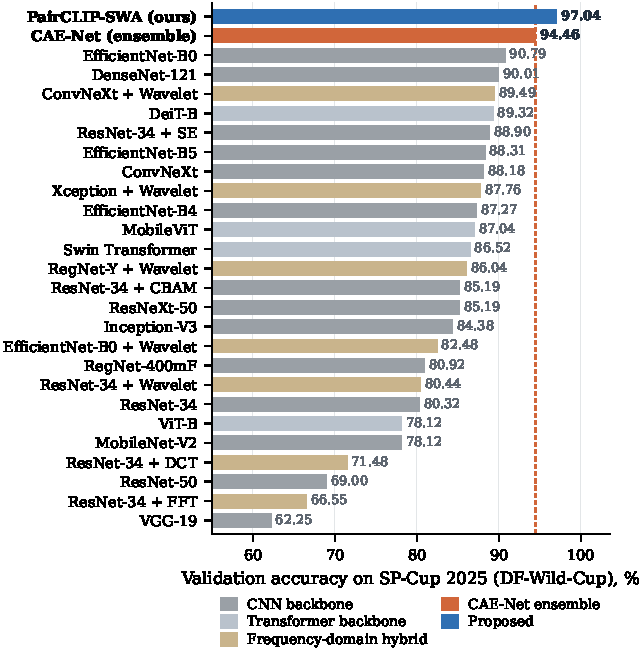
\includegraphics[width=\columnwidth]{figures/benchmark_bars.pdf}
\caption{Accuracy on the SP-Cup 2025 validation set for every model reported
on this corpus. Grey, light-blue and tan bars are the spatial, transformer and
frequency-domain baselines of~\cite{bhattacharjee2026caenet}; the dashed line
marks the previous best result. PairCLIP-SWA is the only single-backbone
model above it.}
\label{fig:bars}
\end{figure}

PairCLIP-SWA improves on the previous best result by $2.58$ percentage
points, from $94.46\%$ to $97.04\%$. Because both figures live near the top of
the scale, the more informative statement is the error reduction: the residual
error falls from $5.54\%$ to $2.96\%$, a $46.5\%$ relative reduction, or $79$
of every $3{,}072$ validation images reclassified correctly. Even the
non-averaged checkpoint, at $95.67\%$, exceeds the ensemble. The gap to the
strongest \emph{single} baseline, EfficientNet-B0 at $90.79\%$, is $6.25$
points.

Table~\ref{tab:head2head} gives the direct head-to-head. We report the full
metric suite of~\cite{bhattacharjee2026caenet} alongside ours, marking
unmeasured entries explicitly rather than estimating them.

\begin{table}[!t]
\caption{Head-to-head on the SP-Cup 2025 validation set ($n=3{,}072$). CAE-Net
figures are as published~\cite{bhattacharjee2026caenet}, with the \textbf{fake}
class positive. Entries marked ``n/l'' were not logged in our evaluation runs;
probe-derived estimates for our model are given separately in
Table~\ref{tab:probe}.}
\label{tab:head2head}
\centering
\footnotesize
\begin{threeparttable}
\begin{tabular}{@{}lcc@{}}
\toprule
Metric & CAE-Net~\cite{bhattacharjee2026caenet} & PairCLIP-SWA \\
\midrule
Accuracy (\%)              & $94.46$ & $\best{97.04}$ \\
Errors out of $3{,}072$     & $170$   & $\best{91}$ \\
Precision (\%)             & $93.70$ & n/l \\
Recall (\%)                & $95.60$ & n/l \\
$F_1$ (\%)                 & $94.64$ & n/l \\
AU-ROC (\%)                & $97.60$ & n/l \\
Equal error rate (\%)      & $5.00$  & n/l \\
Average precision (\%)     & $97.71$ & n/l \\
\midrule
Backbones                  & $3$ & $\best{1}$ \\
Forward passes / image     & $3$ & $\best{1}$ \\
Parameters                 & $\best{117.4}$\,M & $304.0$\,M \\
Inference cost (GMACs)\tnote{a} & $\best{24.8}$ & $81.0$ \\
Training stages            & $5$ & $5$ \\
DF-Wild-Cup train gradients & yes & $\best{\text{no}}$ \\
\bottomrule
\end{tabular}
\begin{tablenotes}[flushleft]\footnotesize
\item[a] CAE-Net value as published; ours computed analytically as
$L(4Nd_m^2+2N^2d_m+8Nd_m^2)+N_p\!\cdot\!3\!\cdot\!14^2 d_m$ with $L=24$,
$N=257$, $d_m=1024$. Wall-clock throughput was not benchmarked on identical
hardware and is therefore omitted.
\end{tablenotes}
\end{threeparttable}
\end{table}

The trade-off is explicit and should not be understated: our detector is
$2.59\times$ larger and $3.27\times$ more expensive per image than the
ensemble it outperforms. What it buys, besides accuracy, is architectural
simplicity --- one backbone, one forward pass, no wavelet preprocessing branch,
no fusion-weight tuning --- and the fact that it never saw the target corpus in
training. Fig.~\ref{fig:tradeoff} places both on the accuracy--compute plane.

\begin{figure}[!t]
\centering
\includegraphics[width=\columnwidth]{figures/tradeoff.pdf}
\caption{Accuracy versus inference cost on SP-Cup 2025. Marker area is
proportional to parameter count. Grey markers are the single models and
ensemble variants of~\cite{bhattacharjee2026caenet}. PairCLIP-SWA occupies a
distinct regime: substantially more compute per image, but a single backbone
and a $46.5\%$ lower error rate than the best ensemble.}
\label{fig:tradeoff}
\end{figure}

\subsection{Embedding-Geometry and Clustering Analysis}\label{sec:cluster-results}
We now apply the analysis of Section~\ref{sec:cluster-method} to a random
subsample of $n=1{,}000$ images ($493$ fake, $507$ real) from the SP-Cup 2025
validation set, embedding the $768$-dimensional penultimate features of each
checkpoint into two dimensions with t-SNE.
Fig.~\ref{fig:tsne-compare} shows the three embeddings side by side and
Fig.~\ref{fig:tsne-detail} the full diagnostic panel for the best SWA model.
Table~\ref{tab:geometry} reports the geometry and Table~\ref{tab:probe} the
probe metrics.

\begin{figure*}[!t]
\centering
\includegraphics[width=\textwidth]{figures/tsne_comparison.png}
\caption{t-SNE embeddings of $1{,}000$ SP-Cup 2025 validation images
($493$ fake, $507$ real) under the three checkpoints. Green denotes real and
red fake; crosses mark class centroids. All three produce two coherent
lobes despite the eight distinct generator families present in the corpus.
The two SWA embeddings are visibly more compact and more cleanly bisected than
the non-averaged one, even though their raw separation score is lower
(Table~\ref{tab:geometry}).}
\label{fig:tsne-compare}
\end{figure*}

\begin{figure*}[!t]
\centering
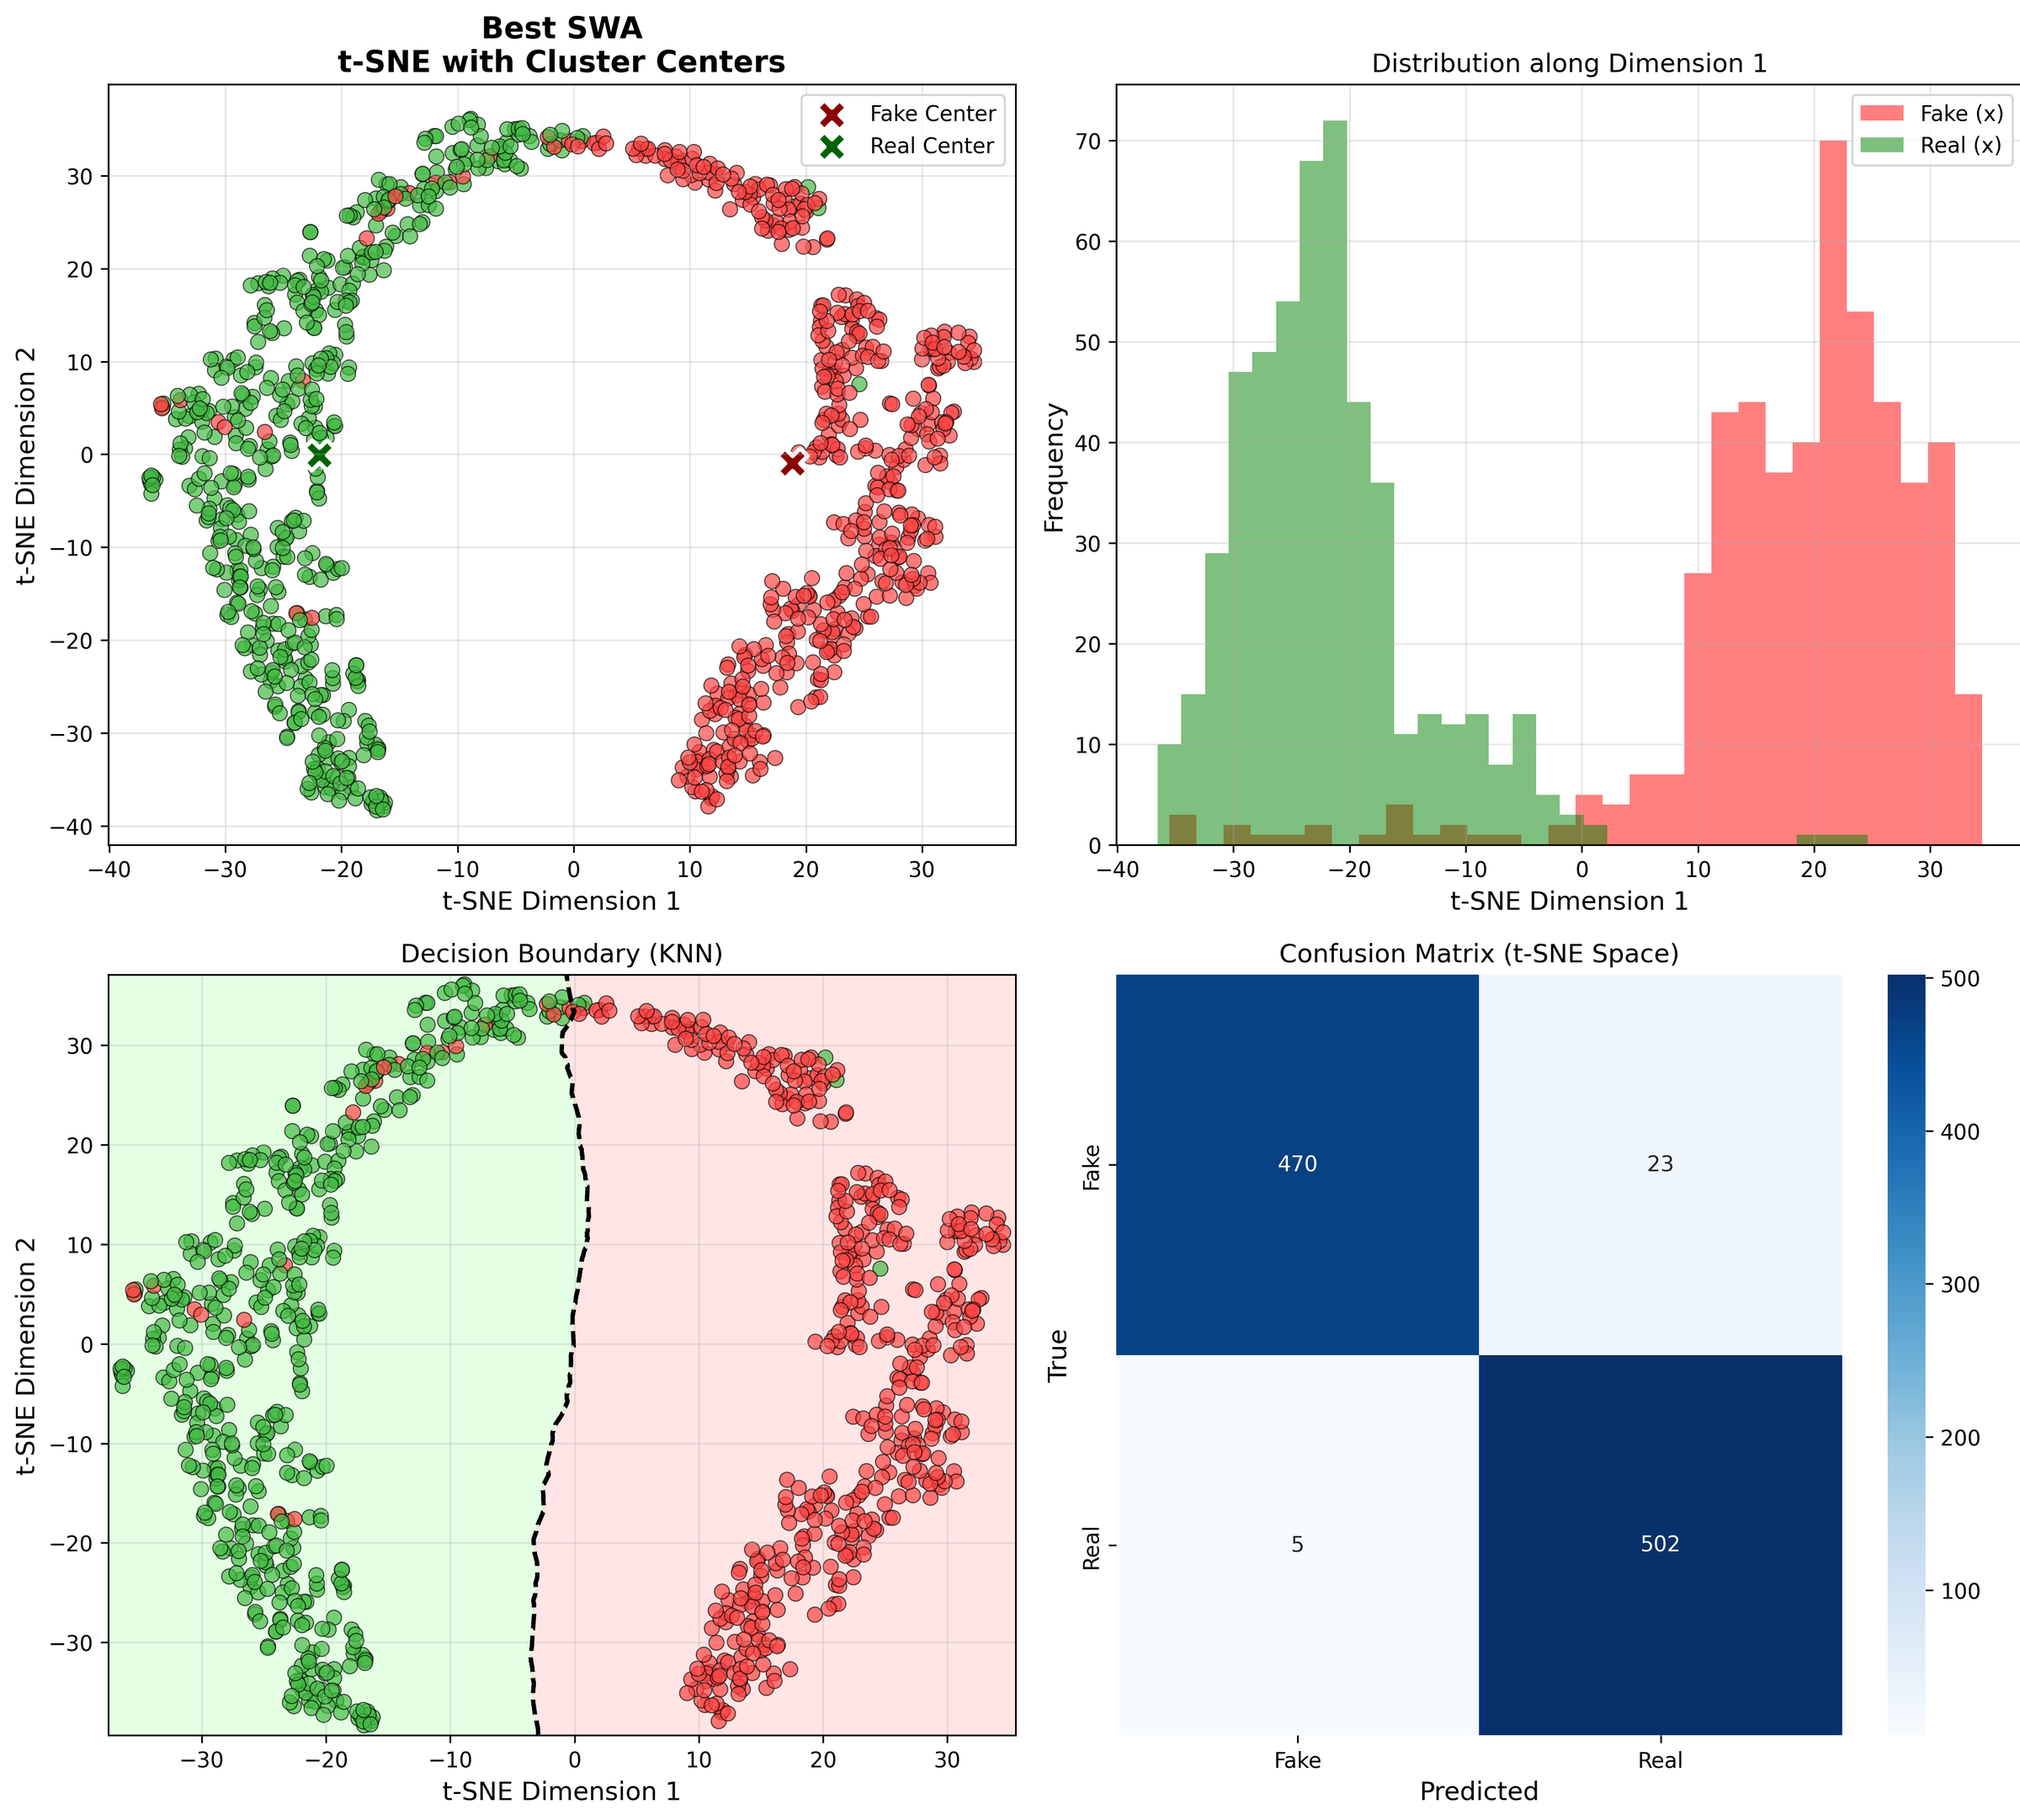
\includegraphics[width=0.78\textwidth]{figures/tsne_best_swa.png}
\caption{Diagnostic panel for the best SWA checkpoint on the SP-Cup 2025
validation subsample. Top left: t-SNE embedding with class centroids. Top
right: marginal distribution along the first t-SNE dimension, which carries
almost all of the class information. Bottom left: k-NN decision boundary in
the embedding. Bottom right: confusion matrix of the probe. The near-complete
separation of the two marginals along dimension~1, and the near-zero
information in dimension~2, indicate that the learned representation encodes
authenticity along an essentially one-dimensional manifold.}
\label{fig:tsne-detail}
\end{figure*}

\begin{table}[!t]
\caption{Cluster geometry in t-SNE space for the SP-Cup 2025 validation
subsample ($n=1{,}000$). $\Delta$ is the inter-centroid distance, $\sigma_c$
the intra-cluster dispersion, and $S=\Delta/(\sigma_f+\sigma_r)$ the
scale-invariant separation score of Eq.~\eqref{eq:sep}.}
\label{tab:geometry}
\centering
\footnotesize
\begin{tabular}{@{}lrrrr@{}}
\toprule
Checkpoint & $\Delta$ & $\sigma_f$ & $\sigma_r$ & $S$ \\
\midrule
Best regular & $43.895$ & $10.697$ & $10.897$ & $\best{2.033}$ \\
Best SWA     & $40.726$ & $10.412$ & $10.721$ & $1.927$ \\
Final SWA    & $39.081$ & $10.318$ & $10.071$ & $1.917$ \\
\bottomrule
\end{tabular}
\end{table}

\begin{table}[!t]
\caption{k-NN probe on the two-dimensional t-SNE embedding of the SP-Cup 2025
validation subsample ($n=1{,}000$), with the \textbf{fake} class positive. The
final column repeats the accuracy of the trained classification head on the
full $3{,}072$-image validation set for reference.}
\label{tab:probe}
\centering
\footnotesize
\begin{tabular}{@{}lrrrrrr@{}}
\toprule
Checkpoint & Acc. & Prec. & Rec. & $F_1$ & MCC & \makecell{Head\\acc.} \\
\midrule
Best regular & $96.00$ & $\best{98.92}$ & $92.90$ & $95.82$ & $0.922$ & $95.67$ \\
Best SWA     & $\best{97.20}$ & $98.95$ & $95.33$ & $97.11$ & $\best{0.945}$ & $97.04$ \\
Final SWA    & $\best{97.20}$ & $98.54$ & $\best{95.74}$ & $\best{97.12}$ & $0.944$ & $97.04$ \\
\midrule
\multicolumn{7}{@{}l}{\emph{Probe confusion matrices (TP/FN/FP/TN, fake positive)}}\\
Best regular & \multicolumn{6}{l}{$458$ / $35$ / $5$ / $502$} \\
Best SWA     & \multicolumn{6}{l}{$470$ / $23$ / $5$ / $502$} \\
Final SWA    & \multicolumn{6}{l}{$472$ / $21$ / $7$ / $500$} \\
\bottomrule
\end{tabular}
\end{table}

\begin{figure*}[!t]
\centering
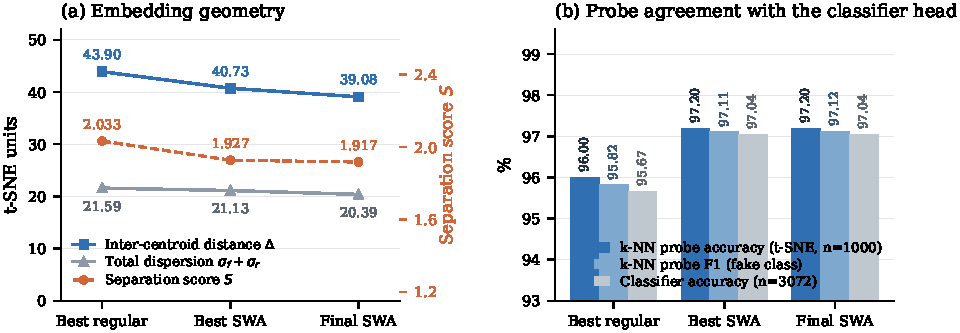
\includegraphics[width=\textwidth]{figures/embedding_geometry.pdf}
\caption{(a) Embedding geometry across checkpoints. Weight averaging
contracts both the inter-centroid distance $\Delta$ and the intra-cluster
dispersion $\sigma_f+\sigma_r$, and the former contracts faster, so the raw
separation score $S$ \emph{decreases}. (b) Nonetheless the k-NN probe on the
same embedding and the trained classification head both \emph{improve},
and agree to within $0.16$ percentage points --- evidence that $S$ measures
cluster spread rather than decision-boundary quality.}
\label{fig:geometry}
\end{figure*}

Four findings emerge.

\textbf{(i) The probe tracks the head.} Probe accuracy on $1{,}000$ images
($97.20\%$) and head accuracy on the full $3{,}072$ ($97.04\%$) differ by
$0.16$ percentage points, and the ordering of the three checkpoints is
identical under both. A two-dimensional nonlinear compression of the
representation therefore retains essentially all of the class information the
linear head uses. This is a strong statement about the representation: the
authenticity signal is not encoded in a fragile high-dimensional direction but
in the global arrangement of the embedding.

\textbf{(ii) Separation and accuracy move in opposite directions.} The best
regular checkpoint has the \emph{highest} separation score
($S=2.033$) and the \emph{lowest} accuracy. Fig.~\ref{fig:geometry}(a)
explains why: averaging contracts $\Delta$ from $43.90$ to $39.08$ ($-11.0\%$)
while contracting the pooled dispersion only from $21.59$ to $20.39$
($-5.6\%$), so the ratio falls. But $S$ is a statement about how far apart and
how spread out the two point clouds are; it says nothing about how cleanly the
region \emph{between} them is bisected. The probe confusion matrices settle
the question: averaging removes $14$ of the $35$ fake-side errors while
leaving the real side untouched. The practical lesson --- relevant to any
paper that reports cluster indices as evidence of representation quality --- is
that global separability indices and boundary quality are distinct
measurements, and the former is not a proxy for the latter.

\textbf{(iii) The error budget is asymmetric.} Every checkpoint is markedly
more reliable on real images than on fake ones: probe specificity is
$98.6$--$99.0\%$ against a recall of $92.9$--$95.7\%$. The detector's residual
weakness is missed forgeries, not false alarms. For a deployment that
prioritizes recall --- content moderation, say --- the decision threshold
of~\eqref{eq:head} can be shifted toward the fake class, trading the plentiful
specificity margin for recall.

\textbf{(iv) Authenticity is essentially one-dimensional.} The marginal
histograms in Fig.~\ref{fig:tsne-detail} show near-complete separation along
t-SNE dimension~1 and near-total overlap along dimension~2. Whatever the
eight generator families of DF-Wild-Cup have in common, the fine-tuned tower
has collapsed it onto a single dominant axis --- consistent with the
observation of~\cite{ojha2023universal} that CLIP's manifold contains a
largely generator-agnostic ``syntheticity'' direction.

% =========================================================================
\section{Discussion, Ablation and Limitations}\label{sec:discussion}
% =========================================================================

\subsection{Ablation: What Does the Weight Average Buy?}
Table~\ref{tab:main} is itself a controlled ablation of the averaging stage,
since the averaged and non-averaged checkpoints come from the same trajectory,
the same data and the same schedule and differ only in
Eq.~\eqref{eq:swa}. Collecting the three splits, the terminal average is worth
$+1.37$ points on DF-Wild-Cup, $+5.91$ points on the OpenForensics held-out
test partition, and $-0.76$ points on the OpenForensics validation partition.

The sign pattern is the entire result. Averaging displaces the solution
towards the centre of a wide basin~\cite{izmailov2018swa}. On the split used
for selection, the endpoint is by construction the better solution --- it was
chosen for that --- so centring costs a little accuracy. On any split not used
for selection, the perturbed loss surface no longer has its optimum at that
endpoint, and the centred solution is closer to the new optimum than a
solution sitting near a wall of the basin. The magnitude of the effect scales
with the severity of the shift: $-0.76$ points where there is no shift,
$+5.91$ where there is a within-corpus sampling shift, $+1.37$ on a genuinely
different corpus.\footnote{The DF-Wild-Cup gain is smaller than the
OpenForensics test gain not because the shift is milder --- it is far more
severe --- but because the non-averaged baseline there was itself selected on
DF-Wild-Cup, so its starting point is already tuned to that distribution.}
Since the operation adds no parameters, no forward passes and no
architectural change, a practitioner who cares about deployment rather than
leaderboard position should prefer the terminal average essentially always.

\subsection{Validation Accuracy Is a Poor Deployment Proxy}
The most consequential finding of this study is methodological. On the
OpenForensics validation partition the best-regular and best-SWA checkpoints
are the clear winners at $98.43\%$, ahead of the terminal average at
$97.67\%$; a practitioner following standard model-selection practice would
ship them. On the held-out test partition those same checkpoints reach
$88.85\%$ while the rejected terminal average reaches $94.76\%$. Selection on
validation accuracy would therefore have chosen the model that makes
\emph{2.1$\times$ as many errors} in deployment.

The failure is legible in the per-class decomposition of
Fig.~\ref{fig:valtest}(b). The validation-selected model does not degrade
uniformly; it degrades entirely on one class, retaining $98.67\%$ fake-class
recall while its specificity falls to $78.88\%$. Scalar accuracy on a balanced
validation split is blind to this because the two classes are equally
weighted and the pathology only manifests when the real-class distribution
shifts. Two practical recommendations follow. First, model selection for
forensic detectors should be performed on balanced accuracy or MCC computed on
a partition disjoint from the one used for early stopping, not on scalar
accuracy on the early-stopping partition itself. Second, per-class recall
should be reported alongside accuracy as a matter of course; had we reported
only Table~\ref{tab:main}, the $21.1\%$ false-positive rate on genuine test
photographs would have been invisible.

We note that this observation also qualifies our own SP-Cup result. The
figures in Table~\ref{tab:spcup} for both PairCLIP-SWA and
CAE-Net~\cite{bhattacharjee2026caenet} are measured on the split that each
system used for selection, and the analysis here suggests such figures should
be treated as upper bounds on deployment performance rather than estimates of
it.

\subsection{Computational Complexity}
The forward cost of the detector is dominated by the $24$ transformer blocks.
For $N=N_p+1$ tokens of width $d_m$, block $\ell$ costs
$4Nd_m^2$ multiply--accumulates (MACs) for the four projections,
$2N^2d_m$ for the attention matrices, and $8Nd_m^2$ for the expansion-$4$ MLP:
\begin{equation}
\mathrm{MACs}=L\big(12Nd_m^2+2N^2d_m\big)+N_p\cdot 3\cdot 14^2\cdot d_m .
\label{eq:macs}
\end{equation}
With $L=24$, $N=257$, $d_m=1024$, $N_p=256$ this evaluates to
$81.0$ GMACs ($162.0$ GFLOPs) per image, against $24.8$ as reported for
CAE-Net. Memory is $1{,}160$\,MB in \texttt{float32} and $580$\,MB in
\texttt{float16}, against $448$\,MB for the ensemble. Training cost is far
more favourable than these figures suggest, because only $8.3\%$ to $58.0\%$
of parameters ever receive gradients (Table~\ref{tab:params}), so optimizer
state and activation-gradient memory are a fraction of what full fine-tuning
would demand. The quadratic term $2N^2d_m$ contributes only $4.0\%$ of the
total at this resolution, so cost scales close to linearly in token count ---
relevant if higher input resolutions are pursued, as suggested in
Section~\ref{sec:conclusion}. Pair mining is a one-off preprocessing cost of
$O(n_rn_fd)$ MACs plus $n_r+n_f$ CLIP forward passes, amortized over all
subsequent training runs.

\subsection{Why Content Balancing Should Matter}
We can state the argument for Stage~1 sharply even though we cannot, with the
present experiments, isolate its contribution. A classifier trained on a
corpus where $p(c\mid y{=}1)\neq p(c\mid y{=}0)$ has two routes to low
training loss: the manipulation factor $m$, which transfers, and the content
factor $c$, which does not. Empirical risk minimization has no preference
between them and will exploit whichever is more linearly accessible ---
typically $c$, since content is high-amplitude and manipulation traces are
not. Matching in CLIP space suppresses the second route by construction,
because the matched partners have, by the definition of the objective
in~\eqref{eq:assignment}, nearly identical semantic descriptors. The
without-replacement constraint is what makes this hold in aggregate rather
than pointwise: with replacement, a handful of semantically generic fakes
would be selected repeatedly and the marginal fake content distribution would
collapse. That said, CLIP similarity is a proxy for content, not content
itself, and the greedy solver returns an approximate matching --- so the
suppression is partial, and the size of the effect is an empirical question we
have not answered here.

\subsection{On the Absence of Weight Decay}
Setting $\lambda=0$ in AdamW is unusual enough to warrant comment. In our
configuration the regularization budget is spent structurally rather than
through a norm penalty: $41.98\%$ of the tower is frozen at all times and
never moves from its pre-trained value; every batch is exactly class-balanced,
which removes a common source of gradient bias; early stopping caps the
effective capacity; and weight averaging performs an implicit smoothing of the
trajectory. Adding an explicit penalty on top of a frozen-prefix schedule
risks pulling the trainable suffix away from the pre-trained
solution --- the very distortion that~\cite{kumar2022finetuning} identifies as
the mechanism by which fine-tuning degrades out-of-distribution accuracy. We
none the less regard the setting as under-explored, and a sweep over $\lambda$
is the first experiment we would run next.

\subsection{Limitations}
We state the limitations of this study plainly.

\begin{enumerate}
\item \textbf{Metric coverage.} Confusion matrices are available for the
OpenForensics splits (Table~\ref{tab:ofmetrics}) but not for the
$3{,}072$-image SP-Cup split, where only scalar accuracy was logged; the
probe-derived values in Table~\ref{tab:probe} are computed on a
$1{,}000$-image subsample in a two-dimensional embedding, not on the
classifier's own decision function. Because probability scores were not
retained, no threshold-free metric --- AU-ROC, equal error rate, average
precision --- is available for any split, so the corresponding rows of
Table~\ref{tab:head2head} remain incomplete and the operating-point
recommendation of Section~\ref{sec:discussion} cannot yet be quantified.

\item \textbf{No component ablation for pair mining.} We have not trained a
control model on an unmatched but count-balanced corpus, so the contribution
of Stage~1 relative to the CLIP backbone and the SWA stage is not separated.
The argument of Section~\ref{sec:discussion} is mechanistic, not empirical.

\item \textbf{Model selection on the evaluation split.} Early stopping and
checkpoint choice use SP-Cup validation accuracy. This is the same protocol
as~\cite{bhattacharjee2026caenet}, which tunes fusion weights on that split,
so the comparison is fair --- but both numbers are optimistic relative to a
truly held-out test partition, and neither should be read as an unbiased
estimate of deployment accuracy.

\item \textbf{Single run.} Our figures come from one training trajectory.
The ensemble baselines in Table~\ref{tab:spcup} are means over five seeds with
standard deviations up to $\pm3.22$; we cannot report a comparable dispersion.

\item \textbf{No adversarial evaluation.} CAE-Net reports FGSM
robustness~\cite{goodfellow2015fgsm} before and after adversarial training. We
have not evaluated PairCLIP-SWA under adversarial perturbation, and large
vision transformers are not intrinsically robust. Any deployment claim must
await that evaluation.

\item \textbf{Small third corpus.} The HF v3 result rests on $26$ images and
carries essentially no statistical weight.

\item \textbf{Cost.} At $304$\,M parameters and $81$ GMACs per image, the
detector is not suited to edge deployment without distillation or pruning.
\end{enumerate}

% =========================================================================
\section{Conclusion and Future Work}\label{sec:conclusion}
% =========================================================================
We asked whether the generalization gains attributed to heterogeneous
convolution--attention ensembles in deepfake detection can instead be obtained
from a single, well-adapted vision--language backbone. On the IEEE SP Cup 2025
(DF-Wild-Cup) benchmark the answer is yes. PairCLIP-SWA --- an OpenCLIP
ViT-L/14 visual tower adapted through a progressively widening block-unfreezing
schedule on a CLIP-mined, content-balanced corpus, and collapsed by stochastic
weight averaging --- reaches $97.04\%$ on the official validation split without
taking a single gradient step on that corpus, against $94.46\%$ for a
three-backbone ensemble trained in-domain. That is a $46.5\%$ relative
reduction in error with one forward pass instead of three, at the cost of
$3.27\times$ more compute per image. On a $39{,}428$-image
OpenForensics-derived benchmark the same recipe converges within eleven epochs
to $98.64\%$ validation accuracy at $98.46\%$ training accuracy, and the
re-evaluated checkpoint scores $98.43\%$ ($\pm0.13$ points at $95\%$
confidence).

The held-out test partition of that benchmark yielded the study's most
consequential result, and it is a cautionary one. The checkpoint that
validation accuracy selects transfers at only $88.85\%$, and $94.0\%$ of its
errors are genuine photographs rejected as forgeries --- a specificity collapse
from $97.83\%$ to $78.88\%$ that scalar accuracy on a balanced validation split
cannot see. The terminal weight average, which validation accuracy \emph{ranks
last}, transfers at $94.76\%$ with a near-symmetric error budget and cuts the
test error by $53.0\%$. Selection on validation accuracy would have shipped the
model making $2.1\times$ as many deployment errors. We therefore recommend that
forensic detectors be selected on per-class criteria --- balanced accuracy or
MCC --- computed on a partition disjoint from the early-stopping split, and that
per-class recall be reported as a matter of course.

Our embedding analysis contributes a methodological caution alongside the
empirical result. Weight averaging \emph{reduced} the inter-centroid
separation score of the t-SNE embedding while \emph{improving} both the k-NN
probe and the classification head; cluster separability indices measure the
spread of class point clouds, not the quality of the boundary between them,
and should not be reported as evidence of the latter. The close agreement
between the two-dimensional probe and the trained head ($0.16$ percentage
points) further indicates that the authenticity signal in an adapted CLIP
representation lies along a dominant, low-dimensional and largely
generator-agnostic axis.

Four directions follow directly. First, the controlled ablation this study
lacks: train matched-corpus and unmatched-corpus models under identical
schedules to quantify Stage~1 in isolation, and sweep the greedy matcher
against an exact Hungarian solution on a tractable subset to bound the
approximation cost. Second, complete the metric and robustness picture --- full
ROC and DET curves, multi-seed dispersion, and FGSM and PGD evaluation with
and without adversarial fine-tuning. Third, address cost: distil the adapted
tower into a ViT-B or EfficientNet student, or apply low-rank adaptation to the
unfrozen suffix, and measure how much of the $97.04\%$ survives. Fourth,
exploit the discarded half of CLIP --- the text tower --- for prompt-conditioned
or open-vocabulary forgery attribution, which would turn a binary detector
into a system that can also say \emph{what kind} of manipulation it has found.

\section*{Acknowledgment}
The authors thank the IEEE Signal Processing Society for organizing the Signal
Processing Cup 2025 and releasing the DF-Wild-Cup dataset, and the maintainers
of the OpenCLIP project for the pre-trained models used in this study.

\bibliographystyle{IEEEtran}
\bibliography{references}

\end{document}
